\documentclass[journal]{new-aiaa}

% Packages
\usepackage[utf8]{inputenc}
\usepackage{amsmath}
\usepackage{bm}
\usepackage{booktabs}
\usepackage[capitalise]{cleveref}
\usepackage{commath}
\usepackage{float}
\usepackage{gensymb}
\usepackage{graphicx}
\usepackage{hyperref}
\usepackage{mathtools}
\usepackage{multicol}
\usepackage{multirow}
\usepackage{longtable,tabularx}
\usepackage{placeins}
\usepackage{siunitx}
\usepackage{subcaption}
\usepackage{textcomp}
\usepackage[dvipsnames]{xcolor}
\usepackage{threeparttable}

% Definitions and commands
\setlength\LTleft{0pt} 
\newcommand{\red}[1]{\textcolor{Red}{#1}}
\newcommand{\eqdef}{=\vcentcolon}
\newcommand{\vect}[1]{\bm{#1}}
\newcommand{\uvec}[1]{\bm{#1}}
\newcommand{\delfrac}[2]{\frac{\partial#1}{\partial#2}}
\newcommand{\delt}[2]{\frac{\partial^2#1}{\partial#2^2}}
\def\tens#1{\bm{#1}}
\def\til#1{\widetilde{#1}}
\def\lb{\left[}
\def\rb{\right]}
\def\lp{\left(}
\def\rp{\right)}
\def\T{\mathsf{T}}
\def\A{\mathcal{A}}
\def\bp{b^+}
\def\B*{\mathcal{B}^*}
\def\Io{\mathcal{I}^{\circ}}
\def\Ithree{\tens{I}_3}
\def\zthree{\tens{0}_3}
\def\axial{\textnormal{axial}}
\def\xo{x_1}
\def\iono{\uvec{\imath}_1^{\circ}}
\def\itwo{\uvec{\imath}_2^{\circ}}
\def\itho{\uvec{\imath}_3^{\circ}}
\def\aone{\uvec{a}_1}
\def\aonetil{\til{a}_1}
\def\dotout{^{\boldsymbol{\cdot}}}
\def\R{\tens{R}}
\def\RT{\R^\T}
\def\Rdot{\dot{\R}}
\def\RTdot{\Rdot^\T}
\def\Rp{\R^+}
\def\RpT{\R^{+^\T}}
\def\Rpdot{\dot{\R}^{+}}
\def\RpTdot{\dot{\R}^{+^\T}}
\def\Ro{\R^{\circ}}
\def\RoT{\R^{\circ^\T}}
\def\Rprime{\R^{\prime}}
\def\Rpprime{\R^{\prime +}}
\def\RpprimeT{\R^{{\prime +}^\T}}
\def\Rb{\R_b}
\def\RbT{\R^T_b}
\def\Rbdot{\dot{\R}_b}
\def\Rbp{\R^{+}_b}
\def\RbpT{\R^{+^\T}_b}
\def\Rbpdot{\dot{\R}^{+}_b}
\def\Rbo{\R^{\circ}_b}
\def\RboT{\R^{\circ^\T}_b}
\def\Rbodot{\dot{\R}^{\circ}_b}
\def\Rz{\R_0}
\def\Rzp{\R^{\prime}_0}
\def\RzpT{\R^{\prime^\T}_0}
\def\RzT{\R^T_0}
\def\Rzz{\R_{0_0}}
\def\RzzT{\Rzz^\T}
\def\Rzo{\R^{\circ}_0}
\def\Rzdot{\dot{\R}_0}
\def\RzdotT{\Rzdot^\T}
\def\RA{\R_A}
\def\RAT{\R^T_A}
\def\RAdot{\dot{\R}_A}
\def\RAo{\R^{\circ}_A}
\def\RAoT{\R^{\circ^\T}_A}
\def\r{\vect{r}}
\def\ro{\r^{\circ}}
\def\rA{\r_A}
\def\rAo{\r^{\circ}_A}
\def\rdot{\dot{\r}}
\def\rdoto{\rdot^{\circ}}
\def\rAdoto{\rdot^{\circ}_A}
\def\rplus{\r^{+}}
\def\rprime{\r^{\prime}}
\def\rpprime{\r^{\prime +}}
\def\rbo{\vect{r}^{\circ}_b}
\def\rbodot{\dot{\vect{r}}^{\circ}_b}
\def\u{\vect{u}}
\def\uT{\u^\T}
\def\uplus{\u^{+}}
\def\uo{\u^{\circ}}
\def\udot{\dot{\u}}
\def\updot{\dot{\u}^{+}}
\def\updotT{\dot{\u}^{+^\T}}
\def\uddot{\ddot{\u}}
\def\uprime{\u^{\prime}}
\def\uprimeT{\u^{\prime^\T}}
\def\upprime{\u^{\prime+}}
\def\upprimeT{\u^{\prime+^\T}}
\def\uhat{\widehat{\u}}
\def\vb{\vect{v}}
\def\vA{\vect{v}_A}
\def\vAo{\vA^{\circ}}
\def\vbdot{\dot{\vect{v}}}
\def\vbplus{\vb^{+}}
\def\vbs{\vb^{*}}
\def\vbsT{\vb^{*^\T}}
\def\vbo{\vb^{\circ}}
\def\vbpdot{\vbdot^{+}}
\def\vP{\vect{v}_P}
\def\vPo{\vP^{\circ}}
\def\vPs{\vP^{*}}
\def\vPsT{\vP^{*^\T}}
\def\om{\vect{\omega}}
\def\omA{\vect{\omega}_A}
\def\omAo{\omA^{\circ}}
\def\omAtil{\til{\omega}_A}
\def\omAtilo{\omAtil^{\circ}}
\def\omp{\om^{+}}
\def\omo{\om^{\circ}}
\def\omdot{\dot{\vect{\omega}}}
\def\omtil{\til{\omega}}
\def\omtilp{\omtil^{+}}
\def\omtilpT{\omtil^{+^\T}}
\def\omtilo{\omtil^{\circ}}
\def\omtildot{\dot{\til{\omega}}}
\def\gam{\vect{\gamma}}
\def\gamp{\gam^{+}}
\def\gampT{\gam^{+^\T}}
\def\gamptil{\til{\gamma}^{+}}
\def\gampdot{\dot{\gam}^{+}}
\def\kap{\vect{\kappa}}
\def\kaptil{\til{\kappa}}
\def\kappdot{\dot{\kap}^{+}}
\def\kapp{\kap^{+}}
\def\kappT{\kap^{+^\T}}
\def\kapptil{\til{\kappa}^{+}}
\def\k{\vect{k}}
\def\kp{\k^{+}}
\def\kpT{\k^{+^\T}}
\def\ktil{\til{k}}
\def\ktilp{\ktil^{+}}
\def\ktilpT{\ktil^{+^\T}}
\def\K{\vect{K}}
\def\Ks{\K^{*}}
\def\Ktil{\til{K}}
\def\Ktils{\Ktil^{*}}
\def\KtilsT{\Ktil^{*^\T}}
\def\kd{\vect{k}_d}
\def\kdtil{\til{k}_d}
\def\kds{\kd^*}
\def\kdtils{\kdtil^*}
\def\xis{\vect{\xi}^{*}}
\def\xisT{\vect{\xi}^{*^\T}}
\def\xitils{\til{\xi}^{*}}
\def\xitilsT{\til{\xi}^{*^\T}}
\def\xio{\vect{\xi}^{\circ}}
\def\etas{\vect{\eta}^*}
\def\etatils{\til{\eta}^*}
\def\etatilsT{\til{\eta}^{*^\T}}
\def\etatile{\til{\eta}_e}
\def\etatilse{\til{\eta}_e^*}
\def\etatiloe{\til{\eta}_e^\circ}
\def\iotas{\tens{\iota}^*}
\def\iotasT{\tens{\iota}^{*^\T}}
\def\V{\vect{V}}
\def\Vs{\V^{*}}
\def\Vo{\V^{\circ}}
\def\VsT{\V^{*^\T}}
\def\Vtils{\til{V}^{*}}
\def\VtilsT{\til{V}^{*^\T}}
\def\Vsdot{\dot{\V}^{*}}
\def\Om{\vect{\Omega}}
\def\Oms{\Om^{*}}
\def\OmsT{\Om^{*^\T}}
\def\Omo{\Om^{\circ}}
\def\Omsdot{\dot{\Om}^{*}}
\def\Omtil{\til{\Omega}}
\def\Omtils{\Omtil^{*}}
\def\Omtilo{\Omtil^{\circ}}
\def\P{\vect{P}}
\def\Pdot{\dot{\P}}
\def\Ps{\P^*}
\def\Pdots{\dot{\P}^*}
\def\Ptils{\til{P}^{*}}
\def\PsT{\P^{*^\T}}
\def\Phats{\widehat{\P}^*}
\def\Hv{\vect{H}}
\def\Hvdot{\dot{\Hv}}
\def\Hvs{\Hv^*}
\def\Hvdots{\Hvdot^*}
\def\HvsT{\Hv^{*^\T}}
\def\Hhats{\widehat{\Hv}^*}
\def\Q{\tens{Q}}
\def\HT{\Q^\T}
\def\Hinv{\Q^{-1}}
\def\HinvT{\Q^{-\T}}
\def\Hdot{\dot{\Q}}
\def\HTdot{\Hdot^\T}
\def\Hp{\Q^{+}}
\def\HpT{\Q^{+^\T}}
\def\Hpinv{\Q^{+^{-1}}}
\def\HpmT{\Q^{+^{-\T}}}
\def\p{\vect{p}}
\def\pprime{\p^{\prime}}
\def\pdot{\dot{\p}}
\def\pddot{\ddot{\p}}
\def\pplus{\p^{+}}
\def\ppdot{\pdot^{+}}
\def\ppprime{\p^{\prime{+}}}
\def\phat{\widehat{\p}}
\def\ptil{\til{p}}
\def\pptil{\til{p}^+}
\def\F{\vect{F}}
\def\Fhat{\widehat{\F}}
\def\Fhats{\Fhat^*}
\def\Fs{\F^*}
\def\FsT{\F^{*^\T}}
\def\Fsprime{\F^{\prime*}}
\def\Ftils{\til{F}^*}
\def\M{\vect{M}}
\def\Mhat{\widehat{\M}}
\def\Mhats{\Mhat^*}
\def\Ms{\M^*}
\def\MsT{\M^{*^\T}}
\def\Msprime{\M^{\prime*}}
\def\f{\vect{f}}
\def\fs{\f^*}
\def\fsT{\f^{*^\T}}
\def\m{\vect{m}}
\def\ms{\m^*}
\def\msT{\m^{*^\T}}
\def\delF{\vect{\delta F}}
\def\delFT{\delF^\T}
\def\delFp{\delF^{\prime}}
\def\delFpT{\delF^{\prime^\T}}
\def\delM{\vect{\delta M}}
\def\delMT{\delM^\T}
\def\delMp{\delM^{\prime}}
\def\delMpT{\delM^{\prime^\T}}
\def\delP{\vect{\delta P}}
\def\delPT{\delP^\T}
\def\delH{\vect{\delta H}}
\def\delHT{\delH^\T}
\def\delFs{\delF^*}
\def\delFsT{\delF^{*^\T}}
\def\delMs{\delM^*}
\def\delMsT{\delM^{*^\T}}
\def\delPs{\delP^*}
\def\delPsT{\delP^{*^\T}}
\def\delHs{\delH^*}
\def\delHsT{\delH^{*^\T}}
\def\delq{\vect{\delta q}}
\def\delqp{\delq^+}
\def\delqs{\delq^*}
\def\delqdots{\dot{\delq}^{*}}
\def\delqdotsT{\dot{\delq}^{*^\T}}
\def\delqsT{\delq^{*^\T}}
\def\delqps{\delq^{\prime*}}
\def\delqpsT{\delq^{{\prime*}^\T}}
\def\dpsi{\vect{\d\psi}}
\def\dpsiT{\dpsi^\T}
\def\dpsis{\dpsi^*}
\def\delpsi{\vect{\delta\psi}}
\def\delpsiT{\delpsi^\T}
\def\delpsip{\delpsi^{\prime}}
\def\delpsipT{\delpsi^{\prime^\T}}
\def\delpsis{\delpsi^*}
\def\delpsisT{\delpsi^{*^\T}}
\def\delpsips{\delpsi^{\prime*}}
\def\delpsipsT{\delpsi^{\prime*^\T}}
\def\delpsidot{\dot{\delpsi}}
\def\delpsisdot{\delpsidot^{*}}
\def\delpsisdotT{\delpsidot^{*^\T}}
\def\delpsitil{\til{\delta\psi}}
\def\delpsitils{\delpsitil^*}
\def\delpsitilps{\til{\delta\psi}^{\prime*}}
\def\delpsitilsT{\delpsitil^{*^\T}}
\def\delpsitilsdot{\dot{\til{\delta\psi}^{*}}}
\def\lamb{\vect{\lambda}}
\def\zv{\vect{0}}
\def\Deltal{\Delta \ell_e}
\def\Deltalinv{\frac{1}{\Deltal}}
\def\dlotwo{\frac{\Deltal}{2}}
\def\intt{\int_{t_1}^{t_2}}
\def\intl{\int_{0}^{\ell}}
\def\d{\textnormal{d}}
\def\RRz{\lp\R\;\Rz\rp}
\def\RRzT{\RRz^\T}
\def\re{\r_e}
\def\vbe{\vect{v}_{e}}
\def\ombe{\vect{\omega}_{e}}
\def\omtilbe{\til{\omega}_{e}}
\def\ue{\u_e}
\def\udote{\udot_e}
\def\uep{\vect{u}^{\prime}_e}
\def\pe{\p_e}
\def\pdote{\pdot_e}
\def\pep{\vect{p}^{\prime}_e}
\def\Vse{\Vs_e}
\def\Vtilse{\til{V}^*_{e}}
\def\Vsdote{\dot{\V}_e^*}
\def\Omse{\Oms_e}
\def\Omsdote{\dot{\Om}_e^*}
\def\Omtilse{\til{\Omega}^*_{e}}
\def\gampe{\gamp_e}
\def\kappe{\kapp_e}
\def\gamptile{\til{\gamma}^{+}_e}
\def\kptile{\til{k}^{+}_e}
\def\kapptile{\til{\kappa}^{+}_e}
\def\Kstile{\til{K}^{*}_e}
\def\Fse{\Fs_e}
\def\Fsep{\vect{F}^{\prime*}_e}
\def\Fstile{\til{\F}_e^*}
\def\Mse{\Ms_e}
\def\Msep{\vect{M}^{\prime*}_e}
\def\Pse{\Ps_e}
\def\Pstile{\til{\P}_e^*}
\def\Pdotse{\dot{\P}_e^*}
\def\Hse{\Hvs_e}
\def\Hdotse{\dot{\Hv}_e^*}
\def\Qe{\Q_e}
\def\HTe{\Q^\T_e}
\def\HinvTe{\Q^{-\T}_e}
\def\fe{\f_e}
\def\me{\m_e}
\def\Re{\R_{e}}
\def\Rdote{\dot{\R}_e}
\def\ReT{\R_{e}^\T}
\def\Rze{\R_{0_e}}
\def\RzeT{\R_{0_e}^\T}
\def\Rzep{\R_{0_e}^\prime}
\def\RRze{\lp\Re\Rze\rp}
\def\RRzeT{\RRze^\T}
\def\xom{x_{1_e}}
\def\xoz{x_{1_0}}
\def\rz{\r_0}
\def\kn{k_{n}}
\def\knt{\kn^2}
\def\kkT{\kp\k^{+^\T}}
\def\varrhoten{\tens{\varrho}}
\def\varrhotenp{\varrhoten^+}
\def\varrhotenpT{\varrhoten^{+^\T}}
\def\varepsten{\tens{\varepsilon}}
\def\varepstenp{\varepsten^+}
\def\varepstenpT{\varepsten^{+^\T}}
\def\Stiff{\mathcal{\tens{S}}^*}
\def\Stiffe{\Stiff_e}
\def\Flex{\mathcal{\tens{C}}^*}
\def\Flexe{\Flex_e}
\def\Mass{\mathcal{\tens{M}}^*}
\def\Masse{\Mass_e}
\def\Damp{\mathcal{\tens{\mu}}^*}
\def\Dampe{\Damp_e}
\def\Fseps{\F^*_{\varepsilon}}
\def\Mseps{\M^*_{\varepsilon}}
\def\Fsd{\Fs_d}
\def\Msd{\Ms_d}
\def\FsdT{\F_d^{*^\T}}
\def\MsdT{\M_d^{*^\T}}
\def\Fsepse{\F^*_{\varepsilon_e}}
\def\Msepse{\M^*_{\varepsilon_e}}
\def\Fsepsdot{\dot{\F}^*_{\varepsilon}}
\def\Msepsdot{\dot{\M}^*_{\varepsilon}}
\def\Fsepsdote{\dot{\F}^*_{\varepsilon_e}}
\def\Msepsdote{\dot{\M}^*_{\varepsilon_e}}
\def\deltaWe{\overline{\delta\mathcal{W}}_{\text{ext}}}
\def\deltaWd{\overline{\delta\mathcal{W}}_{\text{d}}}
\def\deltaA{\overline{\delta\mathcal{A}}}
\def\Sys{\mathcal{\vect{G}}}
\def\X{\vect{X}}
\def\Xo{\vect{X}_1}
\def\Xi{\X_i}
\def\Xdot{\dot{\X}}
\def\Xdoti{\dot{\X}_i}
\def\Xbar{\bar{{\X}}}
\def\Xv{\check{{\X}}}
\def\Xvdot{\dot{\Xv}}
\def\Xz{\X_0}
\def\Resi{\vect{R}_i}
\def\Reso{\vect{R}_1}
\def\JacSys{\tens{J}}
\def\JacSysi{\JacSys_i}
\def\MassSys{\tens{M}}
\def\dt{\Delta t}
\def\ydot{\dot{y}}
\def\yddot{\ddot{y}}
\def\todt{\frac{2}{\dt}}
\def\fg{\f_g}
\def\mg{\m_g}
\def\fgo{\fg^{\circ}}
\def\mgo{\mg^{\circ}}
\def\g{g}
\def\phiscl{\mathring{\phi}}
\def\phiext{\breve{\phi}}
\def\pscaled{\mathring{\p}}
\def\pscalednorm{\mathring{p}}
\def\ptilscl{\til{\mathring{p}}}
\def\pscalede{\pscaled_e}
\def\pext{\breve{\p}}
\def\pextnorm{\breve{p}}
\def\ptilext{\til{\breve{p}}}
\def\pextdot{\dot{\pext}}
\def\pexte{\pext_e}
\def\Fu{\mathtt{\vect{F}}_{u_e}}
\def\Fupi{\mathtt{\vect{F}}_{u_i}^\rightarrow}
\def\Fumj{\mathtt{\vect{F}}_{u_j}^\leftarrow}
\def\Fumk{\mathtt{\vect{F}}_{u_k}^\leftarrow}
\def\Fum{\Fu^\leftarrow}
\def\Fup{\Fu^\rightarrow}
\def\Fump{\Fu^{\leftrightarrows}}
\def\Fumone{\mathtt{\vect{F}}^\leftarrow_{u_1}}
\def\FupN{\mathtt{\vect{F}}^\rightarrow_{u_N}}
\def\Fupe{\Fu^\rightarrow}
\def\Fumepone{\mathtt{\vect{F}}_{u_{e+1}}^\leftarrow}
\def\Fp{\mathtt{\vect{F}}_{p_e}}
\def\Fppi{\mathtt{\vect{F}}_{p_i}^\rightarrow}
\def\Fpmj{\mathtt{\vect{F}}_{p_j}^\leftarrow}
\def\Fpmk{\mathtt{\vect{F}}_{p_k}^\leftarrow}
\def\Fpm{\Fp^\leftarrow}
\def\Fpp{\Fp^\rightarrow}
\def\Fpmp{\Fp^{\leftrightarrows}}
\def\Fpmone{\mathtt{\vect{F}}^\leftarrow_{\psi_1}}
\def\FppN{\mathtt{\vect{F}}^\rightarrow_{\psi_N}}
\def\Fppe{\Fp^\rightarrow}
\def\Fpmepone{\mathtt{\vect{F}}_{\psi_{e+1}}^\leftarrow}
\def\FF{\mathtt{\vect{F}}_{F_e}}
\def\FFpi{\mathtt{\vect{F}}_{F_i}^\rightarrow}
\def\FFmj{\mathtt{\vect{F}}_{F_j}^\leftarrow}
\def\FFmk{\mathtt{\vect{F}}_{F_k}^\leftarrow}
\def\FFm{\FF^\leftarrow}
\def\FFp{\FF^\rightarrow}
\def\FFmp{\FF^{\leftrightarrows}}
\def\FFmone{\mathtt{\vect{F}}^\leftarrow_{F_1}}
\def\FFpN{\mathtt{\vect{F}}^\rightarrow_{F_N}}
\def\FFpe{\FF^\rightarrow}
\def\FFmepone{\mathtt{\vect{F}}_{F_{e+1}}^\leftarrow}
\def\FM{\mathtt{\vect{F}}_{M_e}}
\def\FMpi{\mathtt{\vect{F}}_{M_i}^\rightarrow}
\def\FMmj{\mathtt{\vect{F}}_{M_j}^\leftarrow}
\def\FMmk{\mathtt{\vect{F}}_{M_k}^\leftarrow}
\def\FMm{\FM^\leftarrow}
\def\FMp{\FM^\rightarrow}
\def\FMmp{\FM^{\leftrightarrows}}
\def\FMmone{\mathtt{\vect{F}}^\leftarrow_{M_1}}
\def\FMpN{\mathtt{\vect{F}}^\rightarrow_{M_N}}
\def\FMpe{\FM^\rightarrow}
\def\FMmepone{\mathtt{\vect{F}}_{M_{e+1}}^\leftarrow}
\def\FV{\mathtt{\vect{F}}_{V_e}}
\def\FO{\mathtt{\vect{F}}_{\Omega_e}}

% Title page
\title{Low-order modeling strategies for the straight and swept Pazy wings}

\author{Luiz G. P. dos Santos\footnote{Postdoctoral Researcher, Department of Mechanical Engineering, luizpancini@usp.br}}
\author{João P. T. P. dos Santos\footnote{PhD Candidate, Department of Mechanical Engineering, joaoptpsantos@usp.br}}
\author{Flávio D. Marques\footnote{Associate Professor, Department of Mechanical Engineering, fmarques@sc.usp.br}}
\affil{São Carlos School of Engineering, University of São Paulo,  São Carlos, São Paulo, 13566590, Brazil}
\author{Guilherme R. Begnini\footnote{Associate Professor, Department of Mechanical Engineering, @ufba.br}}
\affil{Federal University of Bahia, Salvador, Bahia, 40210630, Brazil}

\begin{document}

\maketitle

% Abstract
\begin{abstract}
Here goes the abstract.
\end{abstract}

% Manuscript
\section{Introduction}
\lettrine{I}{n} recent years, \dots

The Pazy wing represents a challenging case for aeroelastic modeling due to its high flexibility and complex aerodynamic interactions. In the present work, the modeling of the Pazy is carried out using the Julia package AeroBeams.jl.

In contrast to previous beam modeling strategies of the Pazy, lead by Riso et al. \cite{riso2021correlations,riso2022low} and adopted by most of the community \cite{ritter2026large}, the wingtip rod is modeled not as an inertia attached to the main wing's tip, but as a separate beam connected to it. As will be shown in the following sections, this approach allows for a more accurate representation of the post-flutter dynamics of the system, which is influenced by the flexibility of the wingtip rod itself. Yet for modal, steady and flutter analyses, the so-called inertial modeling of the wingtip rod, which is also investigated in this work, yields results very close to those obtained with the separate-beam procedure.

\section{Computational framework}

\href{https://github.com/luizpancini/AeroBeams.jl}{AeroBeams} is a computational framework designed to model the aeroelastic behavior of very flexible beam assemblies. It does so through a finite element implementation of the mixed formulation of the geometrically-exact beam theory developed by Hodges \cite{hodges2006nonlinear}, with many modeling decisions inspired by Refs. \cite{hodges1996finite,yu2012gebt,wang2017geometrically}. On the aerodynamics side, it is capable of employing a non-planar unsteady vortex-lattice method (UVLM) in order to capture three-dimensional (3D) effects on largely deformed surfaces, or thin-airfoil theory augmented with dynamic stall models and 3D corrections. In the following sections, each of these modeling aspects is described in more detail.

\subsection{Structural model}

The equations of motion for a beam are obtained through Hamilton's principle, which is written as
\begin{equation}
    \intt\intl \left\{\delta\lp\mathcal{K}-\mathcal{U}\rp+\deltaWd+\deltaWe\right\} \d \xo\;\d t = \deltaA \ \ ,
    \label{eq:hamilton}
\end{equation}
in which $t_1$ and $t_2$ represent initial and final time instances, $l$ is the length of the beam, $\delta$ is the variation operator, $\mathcal{K}$ and $\mathcal{U}$ are the beam's kinetic and strain energies per unit of length, respectively, $\deltaWd$ and $\deltaWe$ are the virtual work of the internal dissipative forces associated with structural damping and of external forces per unit of length, respectively, and $\deltaA$ is the virtual action applied at the beam's ends, at the ends of the time interval. 

Once the expressions for each term in \cref{eq:hamilton} are obtained, the kinematical relationships are adjoined to the statement of the principle as Lagrange multipliers. Then, following \cite{hodges2006nonlinear}, integration by parts with respect to time is performed, leading to
\begin{align}
    \intl &\Biggl\{\Biggr. \delta\uprimeT\lb\RRz\Fs\rb + \delta\uT\lb\lp\R\;\Rz\Ps\rp\dotout+\omtil\RRz\Ps-\f\rb + \delpsipT\lb\RRz\Ms\rb +
    \nonumber \\	&+\delpsiT\lb\lp\R\;\Rz\Hvs\rp\dotout+\omtil\RRz\Hvs+\RRz\lp\Vtils\Ps-\lp\aonetil+\gamptil\rp\Fs\rp-\m\rb + \nonumber \\
    &-\delFpT\u -\delFT\lb\RRz\lp\aone+\gamp\rp-\Rz\aone\rb - \delMpT\p -\delMT\lb\HinvT\Rz\kapp\rb +
    \nonumber \\
    &+\delPT\lb\RRz\Vs-\vb-\omtil\u-\udot\rb + \delHT\lb\RRz\Oms-\om-\Q\,\pdot\rb
    \Biggl.\Biggr\}\;\d \xo \nonumber \\
    &=\lp \delta\uT\Fhat+\delpsiT\Mhat-\delFT\uhat-\delMT\phat \rp\Big|_{0}^{l} \ \ ,
    \label{eq:hamilton_lagrange}
\end{align}
in which $\Fs$, $\Ms$, $\Vs$, $\Oms$, $\Ps$ and $\Hvs$ 
represent the vectors of sectional internal force, internal moment, linear velocity, angular velocity, linear momentum and angular momentum, all measured in the deformed beam frame, respectively, $\gamp$ and $\kapp$ are the force and moment strain vectors, respectively, $\vb$ and $\om$ are the vectors of linear and angular velocity of the body-attached frame, respectively, $\f$ and $\m$ are the vectors of externally applied force and moment (including aerodynamic) per unit length, respectively, $\vect{u}$ is the vector of displacements and $\p$ is the vector of the rotation parameters (for which the Wiener-Milenkovi{\'c} parametrization is used \cite{wang2017geometrically}), both in the body-attached frame, $\R$ and $\Q$ are respectively the rotation tensor and tangent tensor associated to $\p$, $\Rz$ is the rotation tensor from the body-attached frame to the undeformed beam frame, $\delta\u$ and $\delpsi$ are the vectors of virtual translation and virtual rotation, respectively, $\delF$, $\delM$, $\delP$ and $\delH$ are vectors of the variation of the corresponding variables, $\aone=\{1,0,0\}^\T$ is a unit vector, and the notations $\tilde{\lp\cdot\rp}$, $\lp\cdot\rp^\prime$, $\dot{\lp\cdot\rp}$ and $\hat{\lp\cdot\rp}$ respectively denote the vector product operator, derivative with respect to the beam arclength coordinate, derivative with respect to time, and discrete values of the boundary conditions. Note that tensorial quantities resolved in the body-attached basis $\A$ are denoted without any superscript, those in the undeformed and deformed beam bases, $\bp$ and $\B*$, are respectively denoted with $(\cdot)^+$ and $(\cdot)^*$. \Cref{eq:hamilton_lagrange} is a mixed variational statement for the geometrically-exact equations of dynamic equilibrium of Timoshenko beams and kinematical relationships, under the assumption of small strains \cite{hodges2006nonlinear}. However, generalized force-strain and momentum-velocity (i.e., constitutive) relations are needed to close the formulation. The generalized force-strain relations proposed for a linear material are
\begin{align}
    \begin{Bmatrix}
    \Fs \\ \Ms
    \end{Bmatrix}
    = \underbrace{\Stiff
    \begin{Bmatrix}
    \gamp \\ \kapp
    \end{Bmatrix}}_{\text{elastic resultants}}
    + \underbrace{\Damp\Stiff
    \begin{Bmatrix}
    \gampdot \\ \kappdot
    \end{Bmatrix}}_{\text{dissipative resultants}}
    = 
	\begin{Bmatrix}
    \Fseps \\ \Mseps
    \end{Bmatrix}
    + \Damp
    \begin{Bmatrix}
    \Fsepsdot \\ \Msepsdot
    \end{Bmatrix} \ \ ,
    \label{eq:constitutive_stiffness}
\end{align}
in which the $6 \times 6$ matrix $\Stiff=\Stiff(\xo)$ is the beam's sectional stiffness matrix, $\Damp=\Damp(\xo)$ is the Kelvin-Voigt (stiffness-proportional) damping coefficient matrix, and $\Fseps$ and $\Mseps$ are the elastic sectional force and moment resultants, respectively.
The generalized momentum-velocity relationship is given by
\begin{align}
    \begin{Bmatrix}
        \Ps \\ \Hvs
    \end{Bmatrix}
    = \Mass
    \begin{Bmatrix}
        \Vs \\ \Oms
    \end{Bmatrix} \ \ ,
    \label{eq:constitutive_inertia}
\end{align}
in which $\Mass=\Mass(\xo)$ is the sectional inertia matrix.

To develop the finite element model, \cref{eq:hamilton_lagrange} is discretized into two-noded elements, and shape functions of the lowest possible order (constant for generalized velocities and linear for generalized displacements and forces) are assumed for the variations ($\delta$), leading to equilibrium and compatibility equations in a generalized node $C$ connected to elements $i$, $j$, $k$, $\ldots$, given by
\begin{equation}
    \begin{aligned}
        &\Fupi + \Fumj + \Fumk + \ldots - \Fhat_C = \zv \ \ ,
        \\
        &\Fppi + \Fpmj + \Fpmk + \ldots - \Mhat_C = \zv \ \ ,
        \\
        &\FFpi + \uhat_C = \zv \;,\; \FFmj - \uhat_C = \zv \;,\; \FFmk - \uhat_C = \zv \;,\; \ldots \ \ ,
        \\
        &\FMpi + \phat_C = \zv \;,\; \FMmj - \phat_C = \zv \;,\; \FMmk - \phat_C = \zv \;,\; \ldots \ \ ,
        \\
        &\FV = \zv \ \ ,
        \\
        &\FO = \zv \ \ ,
        \label{eq:F_connection_node}
    \end{aligned}
\end{equation}
in which
\begin{align}
    \Fump =& \mp\Re\Rze\Fse - \fe^\leftrightarrows + \dlotwo\lb\lp\Re\Rze\Pse\rp\dotout+\omtilbe\Re\Rze\Pse\rb \ \ ,
    \label{eq_Fu} \\
    \Fpmp =& \mp\Re\Rze\Mse - \me^\leftrightarrows + \dlotwo \lb \lp\Re\Rze\Hse\rp\dotout+\omtilbe\Re\Rze\Hse + \Re\Rze\lp\Vtilse\Pse-\lp\aonetil+\gamptile\rp\Fse\rp \rb \ \ ,
    \label{eq_Fp} \\
    \FFmp =& \pm\ue - \dlotwo\lb\Re\Rze\lp\aone+\gampe\rp-\Rze\aone\rb \ \ , 
    \label{eq_FF} \\
    \FMmp =& \pm\pe - \dlotwo\lb\HinvTe\Rze\kappe\rb \ \ ,
    \label{eq_FM} \\
    \FV =& \Deltal\lp\Re\Rze\Vse-\vbe-\omtilbe\ue-\udote\rp \ \ , 
    \label{eq_FV} \\
    \FO =& \Deltal\lb\lp\Re\Rze\rp\Omse-\ombe-\Qe\pdote\rb \ \ ,
    \label{eq_FO}
\end{align}
where the subscript $\lp\cdot\rp_{e}$ denotes quantities at the center of the element, the superscripts $\lp\cdot\rp^\leftarrow$ and $\lp\cdot\rp^\rightarrow$ designate nodal quantities at the first and second nodes of an element, and $\Deltal$ is the length of an element. Note that the distributed gravitational and aerodynamic loads contribute to the external load vectors $\fe^\leftrightarrows$ and $\me^\leftrightarrows$, and matrices $\Stiff$, $\Mass$ and $\Damp$ are likewise discretized as constant over each element. Moreover, due to the fact that the simplest shape functions were assumed (of which the highest degree is equal to one), the integration may be performed analytically, in such a way that Eqs.~\eqref{eq:F_connection_node} yield a nonlinear algebraic system that may be written as
\begin{align}
    \Sys\lp\X,\Xdot\rp = \zv \ \ ,
    \label{eq:system}
\end{align}
in which $\X$ is the vector of elemental and nodal unknowns, referred to as the array of states. The system of \cref{eq:system} allows several types of analyses, such as steady, dynamic, and stability (eigenvalue problem) about a deformed state. For all of these, a Newton-Raphson nonlinear system solver is used. In dynamic analyses, the generalized-$\alpha$ method for first-order systems developed by \cite{jansen2000generalized} is employed, allowing for numerical damping of the high-frequency modes (those not resolved by the time step) by appropriately choosing the spectral radius at infinite frequency, $\rho_\infty$. In the present work, $\rho_\infty=0.9$ is adopted.

\subsection{Aerodynamic model: UVLM}

\subsection{Aerodynamic model: thin-airfoil theory with dynamic stall}

For every element in the assembly of beams, an aerodynamic surface may be attached, and the developed loads are thereafter distributed to the element's nodes. The airloads in AeroBeams are calculated in the reference frame of the local aerodynamic surface, being composed of normal and tangential forces, and a pitching moment about the beam reference axis. Therefore, note that the lift and drag coefficients, $c_l$ and $c_d$, may be written in terms of the normal and tangential coefficients and the angle of attack, $c_n$, $c_t$ and $\alpha$, through the relations
\begin{align}
    c_l &= c_n\cos{\alpha} + c_t\sin{\alpha} \ \ ,
    \\
    c_d &= c_n\sin{\alpha} - c_t\cos{\alpha} \ \ .
    \label{eq:cl_cd}
\end{align}

The linear unsteady aerodynamic loads are computed through the indicial method in state space form described by \cite{leishman2006principles}. The flow induced by the unsteady wake is used to calculate the unsteady angle of attack of a lifting section attached to the beam element as
\begin{align}
    \alpha = \tan^{-1}\lb-\frac{U_n-\Omega^{*}_1 c\lp \overline{s}-3/4 \rp-\sum_{i=1}^{2}\chi_i}{U_t}\rb \ \ ,
    \label{eq:alpha}
\end{align}
where $c$ is the local chord, $U_t = -V^{*}_2$ and $U_n = -V^{*}_3$ are respectively the tangential and normal relative wind speed components at the beam's reference axis, $\overline{s}$ is the chord-normalized position of that reference axis, $\Omega^{*}_1$ is the sectional pitching angular velocity at the reference axis, and the wake-induced normal velocity component is $\sum_{i=1}^{2}\chi_i$. The aerodynamic states $\chi_i$ are defined by the state equations,
\begin{align}
    \dot{\chi}_i &= -2b_i\beta^2\frac{U}{c}\chi_i + A_i \dot{U}_{n3/4} \ \ ,
    \label{eq:chi_state_eqs}
\end{align}
in which $A_i$ and $b_i$ for $i=1,2$ are the indicial parameters of Wagner's function approximation \cite{leishman2006principles}, $\beta$ is the Prandtl-Glauert compressibility factor, $U=\sqrt{U_t^2+U_n^2}$ is the in-plane airspeed, and $ \dot{U}_{n3/4} = -\dot{V}^{*}_3+\dot{\Omega}^{*}_1 c\lp \overline{s}-3/4 \rp $ is the normal relative wind acceleration at the 3/4-chord.

The circulatory components of the aerodynamic load coefficients induced by the pitch-plunge motion of the aerodynamic surface are therefore described by thin-airfoil theory (without small angles approximations), whereas those induced by a trailing-edge flap deflection and wingtip vortex (induced drag) are added in an ad hoc manner, such that
\begin{align}
    c_n^C &= c_{n_{\alpha}}\sin{\alpha}\cos{\alpha} + c_{n_{\delta}}\delta_f \ \ ,
    \label{eq:cnC}
    \\
    c_m^C &= c_{m_0} + c_n^C\lp\overline{s}-x_{ac}\rp + c_{m_{\delta}}\delta_f \ \ ,
    \label{eq:cmC}
    \\
    c_t^C &= -\frac{c_{d_0}+{c_n^C}^2/(\pi \mathrm{AR})}{\cos{\alpha}} + \eta c_n^C\tan{\alpha} - \frac{c_{d_{\delta}}}{\cos{\alpha}} \delta_f \ \ ,
    \label{eq:ctC}
\end{align}
in which $c_{n_{\alpha}}$ is the normal force coefficient proportionality constant with respect to the angle of attack, $x_{ac}$ is the chord-normalized position of the aerodynamic center, $c_{n_{\delta}}$, $c_{m_{\delta}}$ and $c_{d_{\delta}}$ are the corresponding quantities with respect to the trailing-edge flap deflection angle, $\delta_f$, $c_{m_0}$ is the zero-lift pitching moment coefficient, $c_{d_0}$ and ${c_n^C}^2/(\pi \mathrm{AR})$ are the parasite and induced components of the drag coefficient (where $\mathrm{AR}$ is the surface's aspect ratio), and $\eta$ is the tangential force recovery factor, accounting for viscous drag \cite{leishman2006principles}. Note that the $\sin()$ and $\cos()$ terms in \cref{eq:cnC}, and the $\tan()$ term in \cref{eq:ctC} arise due to the assumption of arbitrarily large angles of attack, and are in conformity with equation 41 of \cite{peters2007state}.

The inertial airload coefficients under incompressible flow conditions given by thin-airfoil theory \cite{leishman2006principles} are
\begin{align}
    c_n^I &= \frac{\pi c \dot{U}_{n_{1/2}}}{2U^2} \ \ ,
    \label{eq:cnI}
    \\
    c_m^I &= -\frac{\pi c}{4U^2}\lb\lp1-2\overline{s}\rp\dot{U}_{n_{1/2}} + \frac{c\dot{\Omega}^{*}_1}{16} + \frac{U\Omega^{*}_1}{2}\rb \ \ ,
    \label{eq:cmI}
\end{align}
in which $\dot{U}_{n_{1/2}}=-\dot{V}^{*}_3+\dot{\Omega}^{*}_1 c\lp \overline{s}-1/2 \rp$ is the normal relative wind acceleration at the midchord. The total airload coefficients are given by the sum of circulatory and inertial components.

\section{Modal matching and calibration}

Through the process of beam condensation described in \cref{sec:beam_condensation}, the Nastran finite element models of the Pazy are reduced to simplified beam representations, characterized by a beam mesh with a specified straight reference axis along the span, and sectional inertia and stiffness matrices defined at each beam element of the main wing. 

Two meshes and their corresponding sets of sectional matrices are considered, namely the nominal and refined meshes, to assess the convergence of the modal properties. The nominal mesh has the same nodal distribution procedure as that of \cite{riso2022low}: the nodes are placed at each rib location, except at the tip, where the last four closely spaced ribs comprise only two nodes, forming a smaller element, yielding a total of 16 nodes. The refined mesh places an additional node at the middle of each element of the nominal mesh, except the tip element, resulting in 30 nodes.

\begin{table}[ht!]
    \centering
    \caption{Unloaded S0 frequencies, beam wingtip rod.}
    \label{tab:S0_beamrod_modal_frequencies}
    \begin{tabular}{c c cc cc}
        \toprule
        \multirow{3}{*}{Mode} & \multirow{3}{*}{Nastran [Hz]} & \multicolumn{4}{c}{AeroBeams} \\
        \cmidrule(lr){3-6}
        & & \multicolumn{2}{c}{Nominal mesh} & \multicolumn{2}{c}{Refined mesh} \\
        \cmidrule(lr){3-4} \cmidrule(lr){5-6}
        & & Frequency [Hz] & $\Delta$ Nastran [\%] & Frequency [Hz] & $\Delta$ Nastran [\%] \\
        \midrule
        OOP1 & 4.19 & 4.20 & 0.09 & 4.19 & 0.02 \\
        OOP2 & 28.48 & 28.58 & 0.35 & 28.50 & 0.07 \\
        T1 & 40.79 & 40.89 & 0.26 & 40.89 & 0.25 \\
        OOP3 & 82.54 & 83.13 & 0.71 & 82.68 & 0.17 \\
        IP1 & 104.97 & 104.99 & 0.02 & 104.93 & $-$0.04 \\
        T2 & 137.48 & 139.16 & 1.22 & 138.90 & 1.03 \\
        R1 & 156.21 & 154.53 & $-$1.07 & 154.53 & $-$1.07 \\
        T3 & 153.56 & 156.72 & 2.06 & 156.16 & 1.69 \\
        OOP4 & 173.11 & 177.17 & 2.35 & 175.91 & 1.62 \\
        R2 & 183.48 & 181.57 & $-$1.04 & 181.57 & $-$1.04 \\
        \bottomrule
    \end{tabular}
\end{table}

\begin{table}[ht!]
    \centering
    \caption{Unloaded S0 frequencies and MAC, for the wingtip rod modeled as a beam (Nastran with flexible rod) and as an inertia (Nastran with rigid rod), refined mesh.}
    \label{tab:S0_modal_rigidtipvsflextip_comparison}
    \begin{tabular}{c cccc cccc}
        \toprule
        \multirow{2}{*}{Mode} & \multicolumn{4}{c}{Beam rod} & \multicolumn{4}{c}{Inertia rod} \\
        \cmidrule(lr){2-5} \cmidrule(lr){6-9}
        & AeroBeams [Hz] & Nastran [Hz] & $\Delta$ [\%] & MAC & AeroBeams [Hz] & Nastran [Hz] & $\Delta$ [\%] & MAC \\
        \midrule
        OOP1 & 4.19 & 4.19 & 0.02 & 1.000 & 4.19 & 4.19 & 0.01 & 1.000 \\
        OOP2 & 28.50 & 28.48 & 0.07 & 1.000 & 28.53 & 28.51 & 0.07 & 1.000 \\
        T1 & 40.89 & 40.79 & 0.25 & 1.000 & 42.13 & 41.99 & 0.33 & 1.000 \\
        OOP3 & 82.68 & 82.54 & 0.17 & 1.000 & 83.15 & 83.02 & 0.16 & 1.000 \\
        IP1 & 104.93 & 104.97 & $-$0.04 & 1.000 & 105.18 & 105.17 & 0.01 & 1.000 \\
        T2 & 138.90 & 137.48 & 1.03 & 0.983 & 164.13 & 162.67 & 0.89 & 0.999 \\
        R1 & 154.53 & 156.21 & $-$1.07 & 1.000 & \multicolumn{4}{c}{---} \\
        T3 & 156.16 & 153.56 & 1.69 & 0.983 & 307.90 & 305.06 & 0.93 & 0.998 \\
        OOP4 & 175.91 & 173.11 & 1.62 & 0.975 & 167.01 & 166.43 & 0.35 & 0.996 \\
        R2 & 181.57 & 183.48 & $-$1.04 & 0.999 & \multicolumn{4}{c}{---} \\
        T4 & 253.98 & 254.32 & $-$0.13 & 0.999 & 456.71 & 451.60 & 1.13 & 0.996 \\
        OOP5 & 283.21 & 281.09 & 0.76 & 0.998 & 280.05 & 278.08 & 0.71 & 1.000 \\
        T5 & 355.70 & 353.77 & 0.55 & 0.997 & 608.99 & 595.80 & 2.21 & 0.994 \\
        OOP6 & 424.72 & 419.48 & 1.25 & 0.999 & 422.38 & 416.82 & 1.33 & 0.999 \\
        \bottomrule
    \end{tabular}
\end{table}

\begin{figure}[ht!]
    \centering
    \begin{subfigure}[b]{0.48\linewidth}
        \centering
        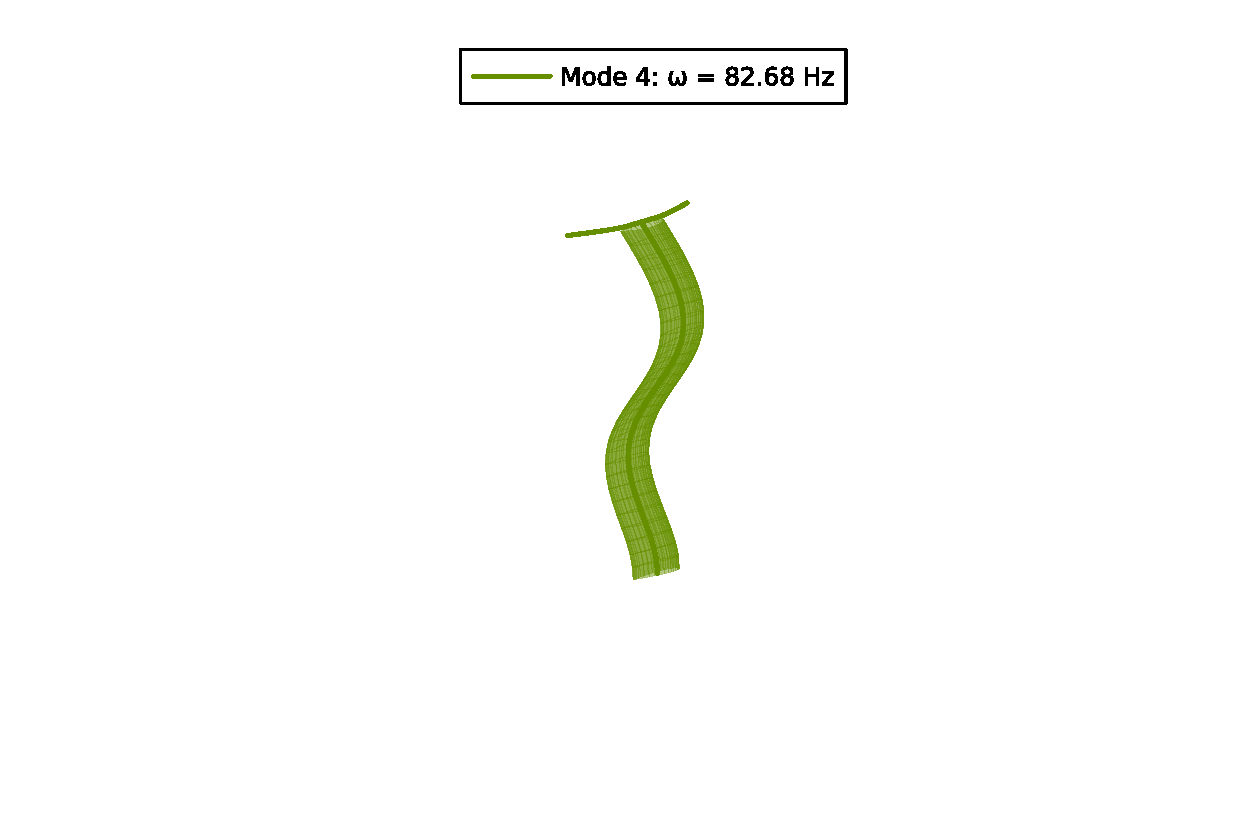
\includegraphics[width=\linewidth, trim={6cm 4cm 6cm 3cm}, clip, keepaspectratio]{figures/S0BeamRodModal_mode4.pdf}
        \caption{AeroBeams, mode 4 (OOP3) -- 82.68 Hz}
        \label{fig:S0_mode4_AeroBeams}
    \end{subfigure}
    \hfill
    \begin{subfigure}[b]{0.48\linewidth}
        \centering
        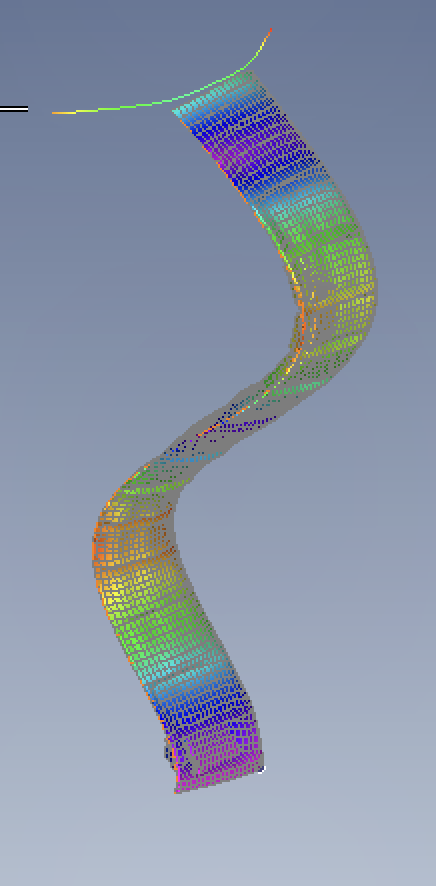
\includegraphics[width=\linewidth, height=0.28\textheight, keepaspectratio]{figures/S0_mode4_Nastran.png}
        \caption{Nastran, mode 4 (OOP3) -- 82.54 Hz}
        \label{fig:S0_mode4_Nastran}
    \end{subfigure}
    \\[1em]
    \begin{subfigure}[b]{0.48\linewidth}
        \centering
        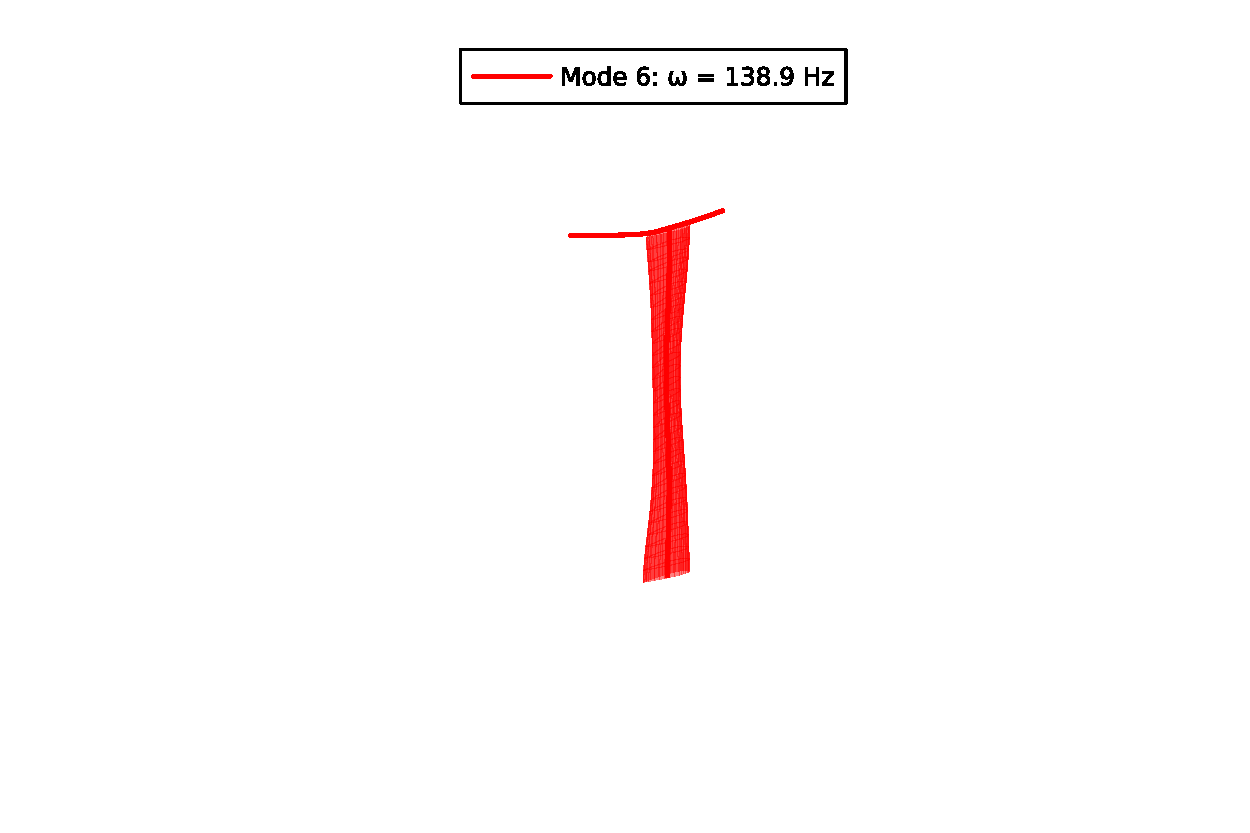
\includegraphics[width=\linewidth, trim={6cm 4cm 6cm 3cm}, clip, keepaspectratio]{figures/S0BeamRodModal_mode6.pdf}
        \caption{AeroBeams, mode 6 (T2) -- 138.90 Hz}
        \label{fig:S0_mode6_AeroBeams}
    \end{subfigure}
    \hfill
    \begin{subfigure}[b]{0.48\linewidth}
        \centering
        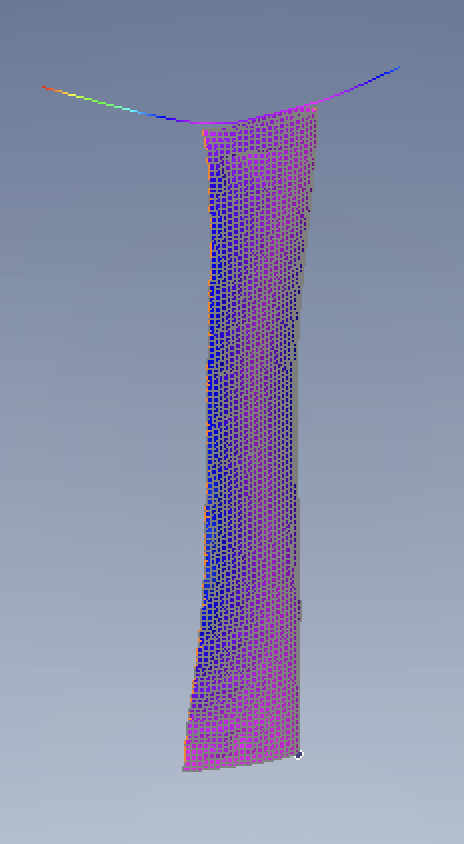
\includegraphics[width=\linewidth, height=0.28\textheight, keepaspectratio]{figures/S0_mode6_Nastran.png}
        \caption{Nastran, mode 6 (T2) -- 137.48 Hz}
        \label{fig:S0_mode6_Nastran}
    \end{subfigure}
    \caption{Mode shapes of the S0 wing, refined mesh.}
    \label{fig:S0_modes_shapes}
\end{figure}

\begin{table}[ht!]
    \centering
    \caption{Unloaded S10 LE and S10 TE frequencies, beam wingtip rod, refined mesh.}
    \label{tab:S10_beamrod_modal_frequencies}
    \setlength{\tabcolsep}{4pt}
    \begin{tabular}{c ccc ccc}
        \toprule
        \multirow{2}{*}{Mode} & \multicolumn{3}{c}{LE} & \multicolumn{3}{c}{TE} \\
        \cmidrule(lr){2-4} \cmidrule(lr){5-7}
        & Nastran [Hz] & AeroBeams [Hz] & $\Delta$ [\%] & Nastran [Hz] & AeroBeams [Hz] & $\Delta$ [\%] \\
        \midrule
        OOP1 & 4.35 & 4.35 & 0.02 & 4.31 & 4.32 & 0.02 \\
        OOP2 & 28.84 & 28.83 & $-$0.03 & 27.05 & 27.02 & $-$0.10 \\
        T1 & 37.83 & 37.59 & $-$0.64 & 38.71 & 38.65 & $-$0.15 \\
        R1 & 64.21 & 64.20 & $-$0.03 & 73.93 & 73.93 & 0.00 \\
        OOP3 & 85.32 & 85.36 & 0.05 & 84.81 & 84.74 & $-$0.08 \\
        T2 & 97.07 & 96.84 & $-$0.24 & 111.07 & 110.42 & $-$0.58 \\
        IP1 & 103.27 & 103.32 & 0.05 & 104.28 & 104.27 & $-$0.01 \\
        OOP4 & 167.41 & 167.78 & 0.22 & 170.09 & 170.51 & 0.25 \\
        T3 & 182.49 & 184.06 & 0.86 & 194.99 & 196.21 & 0.62 \\
        OOP5 & 274.99 & 275.52 & 0.19 & 277.69 & 279.06 & 0.49 \\
        \bottomrule
    \end{tabular}
\end{table}

\begin{table}[ht!]
    \centering
    \caption{Unloaded S20 LE and S20 TE frequencies, beam wingtip rod, refined mesh.}
    \label{tab:S20_beamrod_modal_frequencies}
    \setlength{\tabcolsep}{4pt}
    \begin{tabular}{c ccc ccc}
        \toprule
        \multirow{2}{*}{Mode} & \multicolumn{3}{c}{LE} & \multicolumn{3}{c}{TE} \\
        \cmidrule(lr){2-4} \cmidrule(lr){5-7}
        & Nastran [Hz] & AeroBeams [Hz] & $\Delta$ [\%] & Nastran [Hz] & AeroBeams [Hz] & $\Delta$ [\%] \\
        \midrule
        OOP1 & 4.16 & 4.17 & 0.02 & 4.14 & 4.14 & 0.05 \\
        OOP2 & 28.18 & 28.17 & $-$0.06 & 25.53 & 25.47 & $-$0.20 \\
        T1 & 34.45 & 34.37 & $-$0.25 & 38.32 & 38.26 & $-$0.16 \\
        OOP3 & 83.84 & 83.60 & $-$0.28 & 80.95 & 80.59 & $-$0.44 \\
        R1 & 83.36 & 83.68 & 0.39 & 254.07 & 259.70 & 2.22 \\
        IP1 & 95.02 & 95.07 & 0.05 & 85.38 & 85.41 & 0.04 \\
        IP2 & --- & --- & --- & 106.44 & 106.08 & $-$0.33 \\
        T2 & 131.09 & 130.19 & $-$0.68 & 125.56 & 124.18 & $-$1.10 \\
        OOP4 & 161.57 & 160.74 & $-$0.52 & --- & --- & --- \\
        T3 & 211.98 & 212.89 & 0.43 & 168.75 & 167.72 & $-$0.61 \\
        T4 & 276.74 & 275.03 & $-$0.62 & 188.66 & 189.01 & 0.18 \\
        \bottomrule
    \end{tabular}
\end{table}

\begin{table}[ht!]
    \centering
    \caption{S0, S10 LE, S10 TE, S20 LE and S20 TE frequencies, compared with GVTs \cite{avin2022experimental,revivo2026flutterpost,revivoS10data,revivoS20data}, refined mesh. The wing is upright in a sea-level gravitational field.}
    \label{tab:S0_gvt_comparison}
    \setlength{\tabcolsep}{4pt}
    \begin{threeparttable}
    \begin{tabular}{c c c cc cc}
        \toprule
        \multirow{2}{*}{Configuration} & \multirow{2}{*}{Mode} & \multirow{2}{*}{GVT [Hz]} & \multicolumn{2}{c}{Beam rod} & \multicolumn{2}{c}{Inertia rod\tnote{a}} \\
        \cmidrule(lr){4-5} \cmidrule(lr){6-7}
        & & & Frequency [Hz] & $\Delta$ GVT [\%] & Frequency [Hz] & $\Delta$ GVT [\%] \\
        \midrule
        \multirow{4}{*}{S0} & OOP1 & 4.26 & 4.12 & $-$3.37 & 4.12 & $-$3.37 \\
        & OOP2 & 28.50 & 28.43 & $-$0.25 & 28.45 & $-$0.16 \\
        & T1 & 42.00 & 40.94 & $-$2.52 & 42.13 & 0.30 \\
        & OOP3 & 81.50 & 82.61 & 1.36 & 83.07 & 1.93 \\
        \midrule
        \multirow{4}{*}{S10 LE} & OOP1 & 4.3 & 4.28 & $-$0.49 & 4.28 & $-$0.47 \\
        & OOP2 & 28.9 & 28.76 & $-$0.48 & 29.07 & 0.57 \\
        & T1 & 37.5 & 37.58 & 0.22 & 37.84 & 0.91 \\
        & OOP3 & 86.2 & 85.29 & $-$1.06 & 86.00 & $-$0.23 \\
        \midrule
        \multirow{4}{*}{S10 TE} & OOP1 & 4.3 & 4.24 & $-$1.37 & 4.24 & $-$1.34 \\
        & OOP2 & 27.4 & 26.97 & $-$1.55 & 27.36 & $-$0.16 \\
        & T1 & 38.7 & 38.61 & $-$0.25 & 38.73 & 0.08 \\
        & OOP3 & 85.2 & 84.69 & $-$0.60 & 85.60 & 0.47 \\
        \midrule
        \multirow{4}{*}{S20 LE} & OOP1 & 4.2 & 4.09 & $-$2.62 & 4.09 & $-$2.60 \\
        & OOP2 & 28.4 & 28.09 & $-$1.10 & 28.35 & $-$0.19 \\
        & T1 & 34.0 & 34.36 & 1.07 & 34.50 & 1.48 \\
        & OOP3 & 84.4 & 83.40 & $-$1.18 & 83.58 & $-$0.97 \\
        \midrule
        \multirow{4}{*}{S20 TE} & OOP1 & 4.1 & 4.07 & $-$0.80 & 4.07 & $-$0.80 \\
        & OOP2 & 25.1 & 25.44 & 1.37 & 25.69 & 2.37 \\
        & T1 & 38.1 & 38.20 & 0.26 & 38.31 & 0.56 \\
        & OOP3 & 83.8 & 80.54 & $-$3.89 & 82.07 & $-$2.07 \\
        \bottomrule
    \end{tabular}
    \begin{tablenotes}
        \footnotesize
        \item[a] Tip inertia correction applied to the S10 and S20 configurations.
    \end{tablenotes}
    \end{threeparttable}
\end{table}

\clearpage

\section{Steady aeroelastic response}

% S0

\begin{figure}[ht!]
    \centering
    \begin{subfigure}[b]{0.48\linewidth}
        \centering
        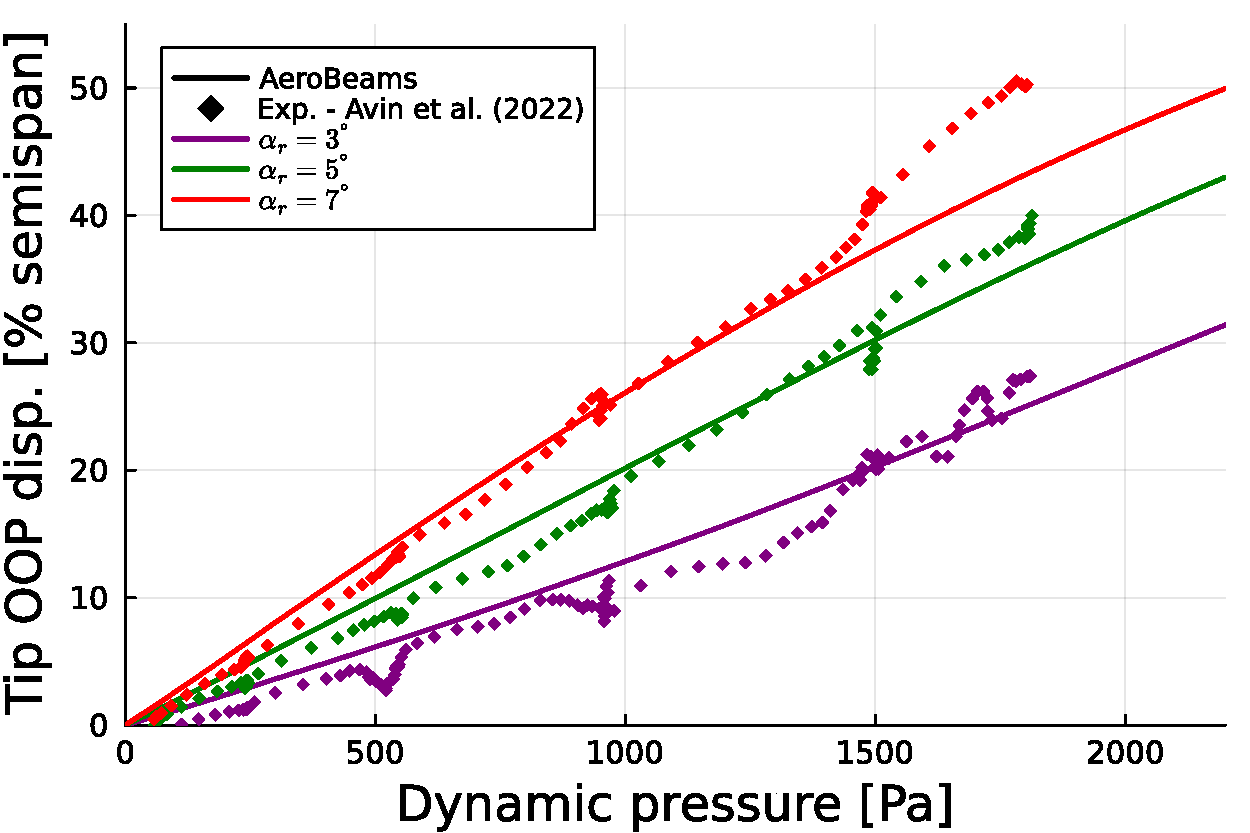
\includegraphics[width=\linewidth]{figures/S0BeamRodPitchRange_tipOOP.pdf}
        \caption{Tip OOP displacement.}
        \label{fig:S0BeamRodPitchRange_tipOOP}
    \end{subfigure}
    \hfill
    \begin{subfigure}[b]{0.48\linewidth}
        \centering
        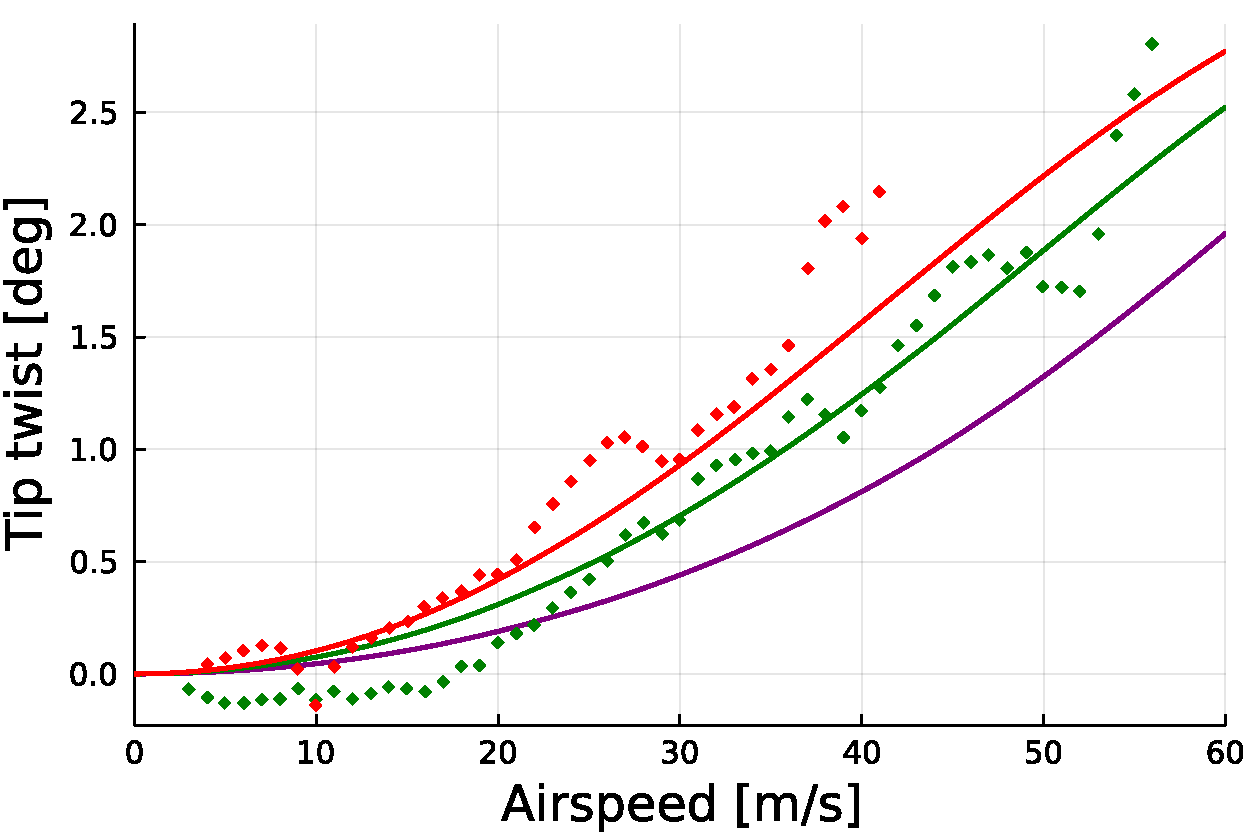
\includegraphics[width=\linewidth]{figures/S0BeamRodPitchRange_tipTwist.pdf}
        \caption{Tip twist.}
        \label{fig:S0BeamRodPitchRange_tipTwist}
    \end{subfigure}
    \caption{S0 beam-rod model: steady response over the pitch range.}
    \label{fig:S0BeamRodPitchRange}
\end{figure}

% S10 and S20

\begin{figure}[ht!]
    \centering
    \begin{subfigure}[b]{0.48\linewidth}
        \centering
        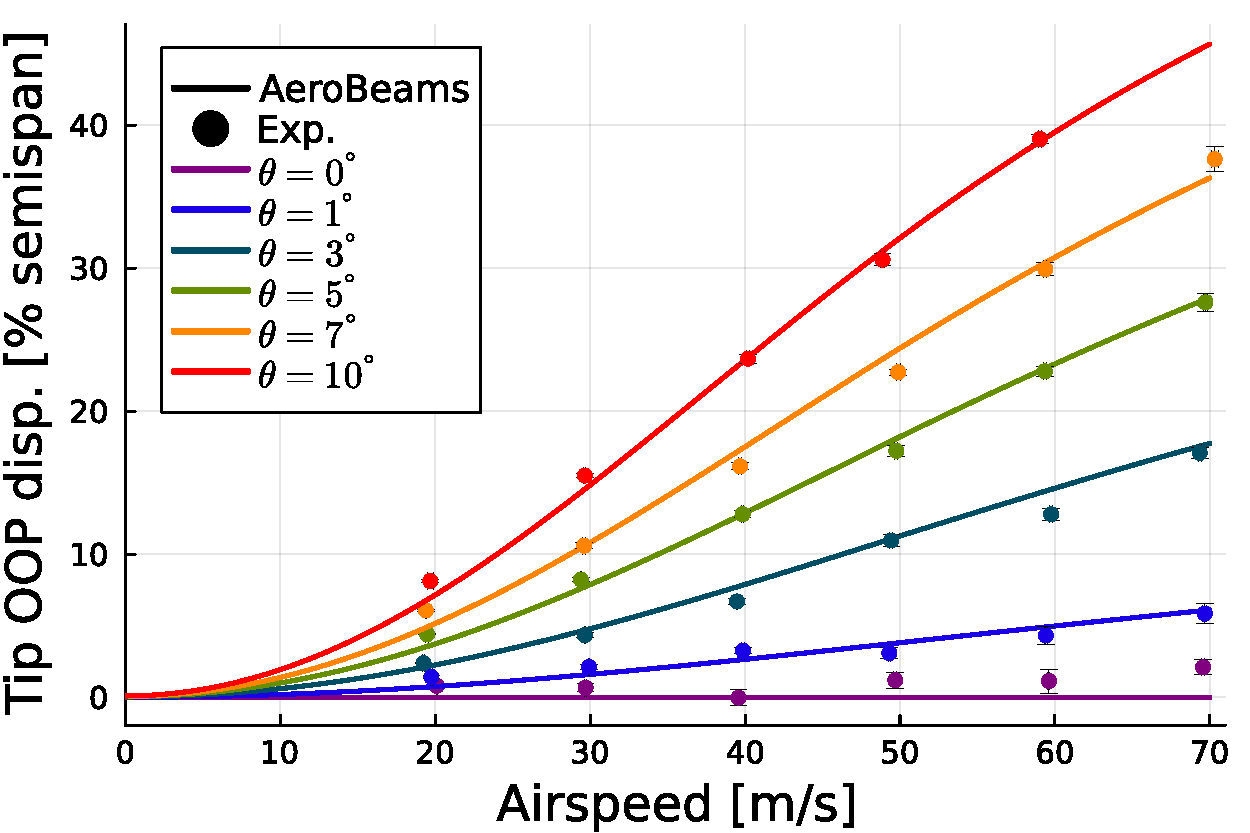
\includegraphics[width=\linewidth]{figures/S10BeamRodSteadyPitchRange_tipOOP.pdf}
        \caption{S10, tip OOP displacement.}
        \label{fig:S10BeamRodSteadyPitchRange_tipOOP}
    \end{subfigure}
    \hfill
    \begin{subfigure}[b]{0.48\linewidth}
        \centering
        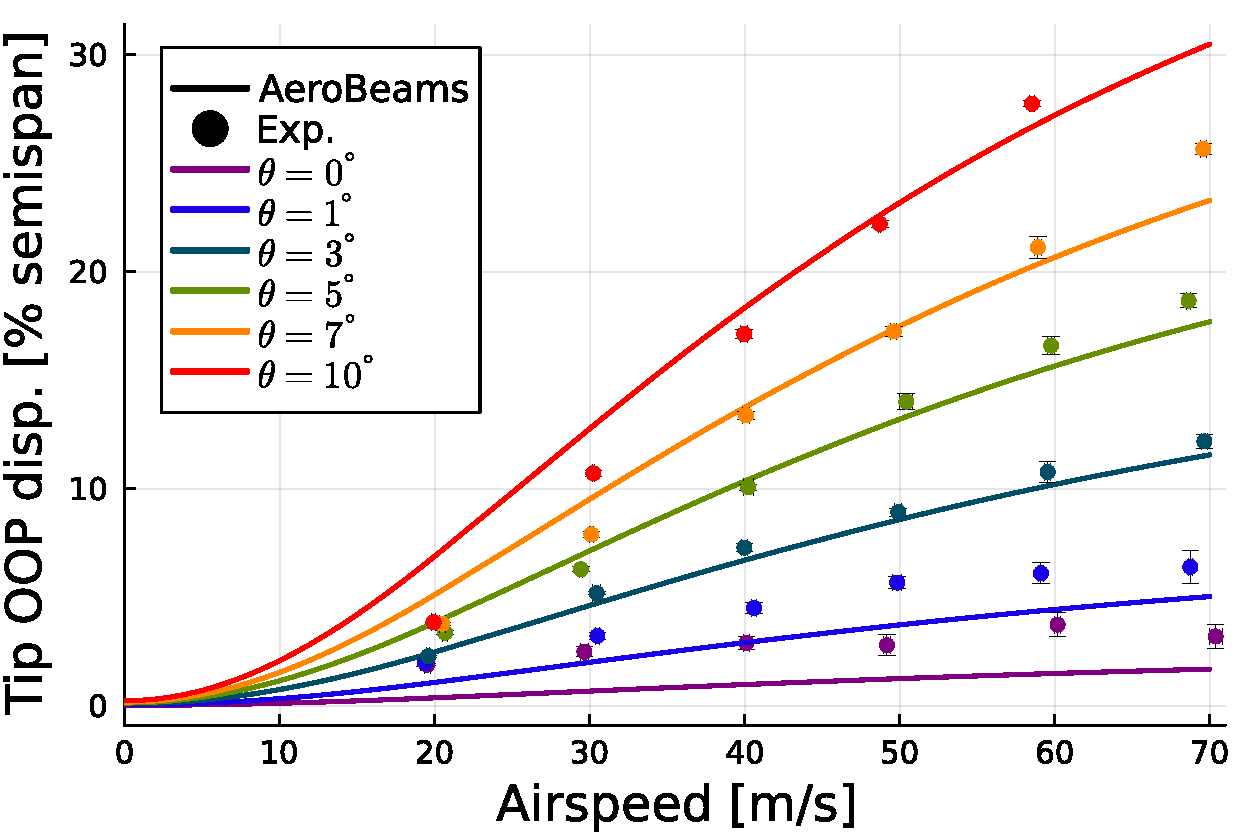
\includegraphics[width=\linewidth]{figures/S20BeamRodSteadyPitchRange_tipOOP.pdf}
        \caption{S20, tip OOP displacement.}
        \label{fig:S20BeamRodSteadyPitchRange_tipOOP}
    \end{subfigure}
    \\[1em]
    \begin{subfigure}[b]{0.48\linewidth}
        \centering
        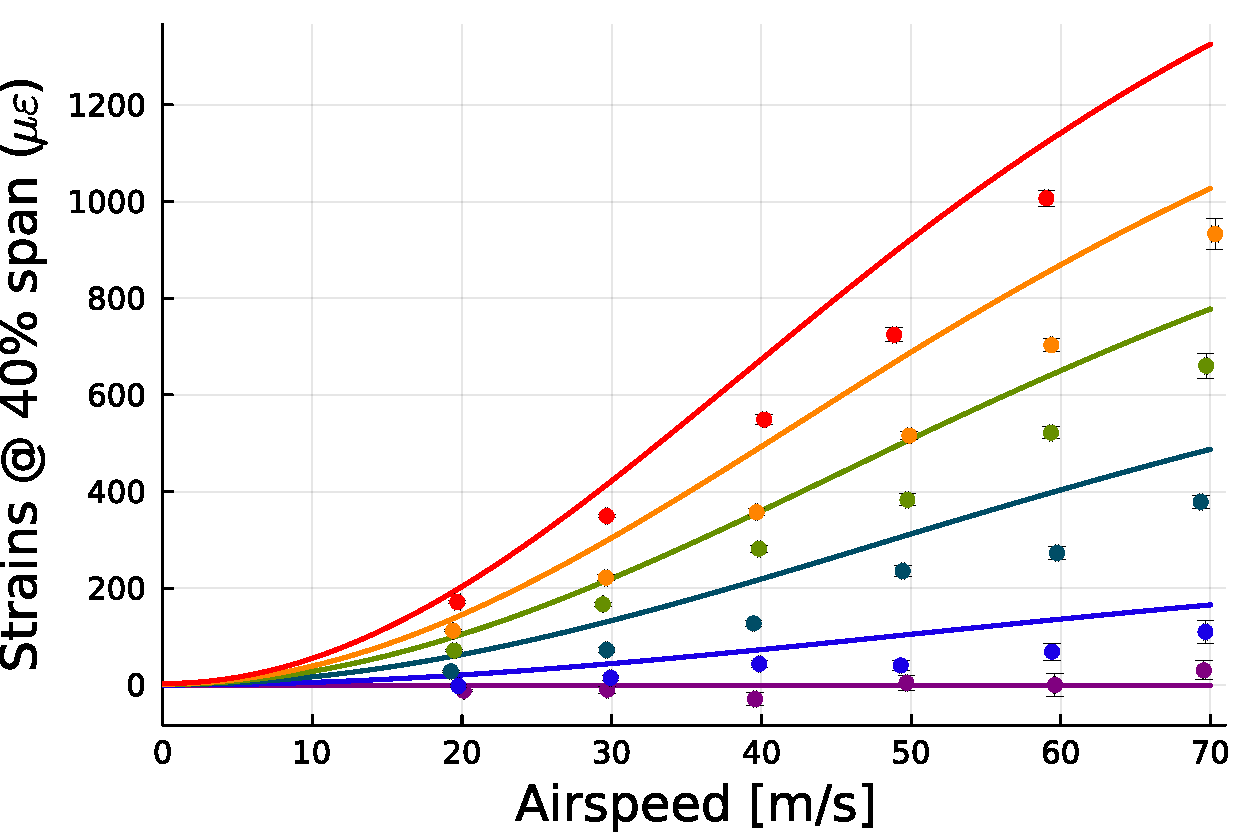
\includegraphics[width=\linewidth]{figures/S10BeamRodSteadyPitchRange_eps.pdf}
        \caption{S10, strains at spar TE (approximately 40\% span).}
        \label{fig:S10BeamRodSteadyPitchRange_eps}
    \end{subfigure}
    \hfill
    \begin{subfigure}[b]{0.48\linewidth}
        \centering
        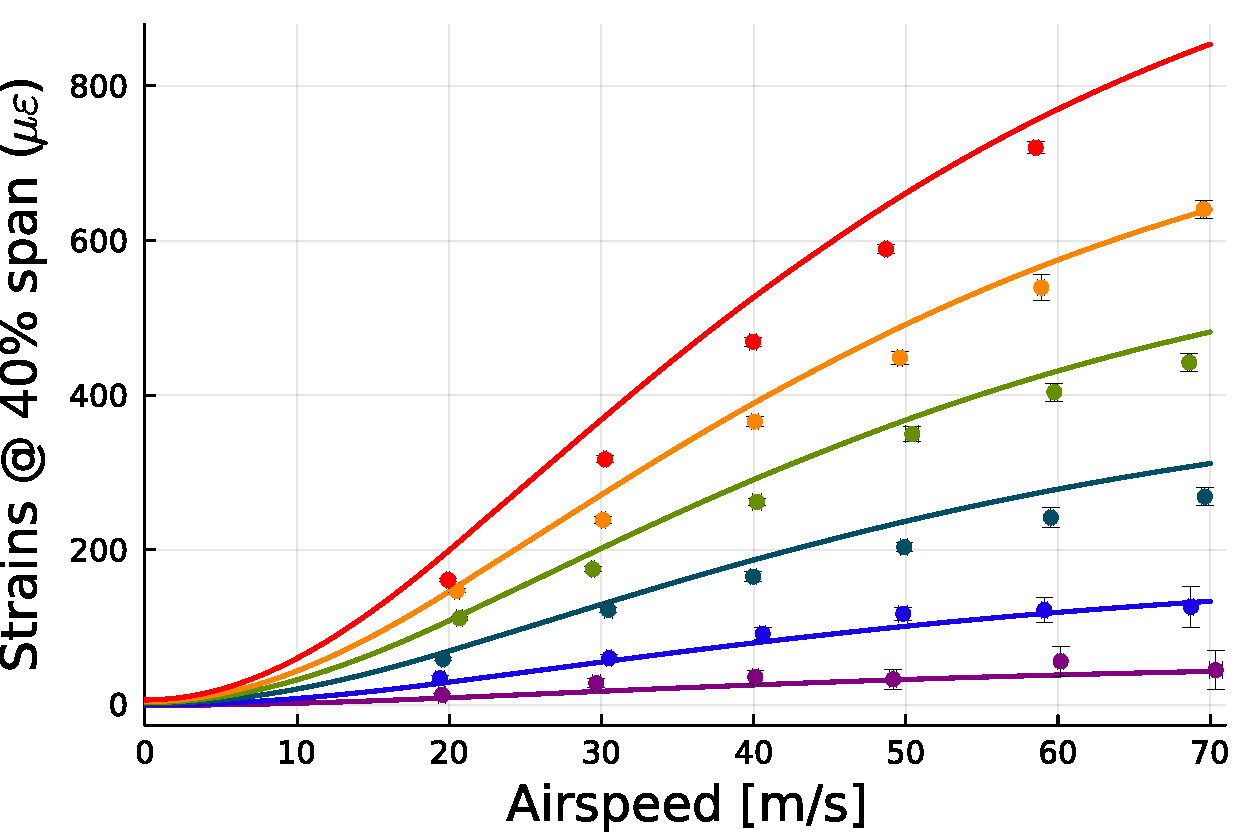
\includegraphics[width=\linewidth]{figures/S20BeamRodSteadyPitchRange_eps.pdf}
        \caption{S20, strains at spar TE (approximately 40\% span).}
        \label{fig:S20BeamRodSteadyPitchRange_eps}
    \end{subfigure}
    \\[1em]
    \begin{subfigure}[b]{0.48\linewidth}
        \centering
        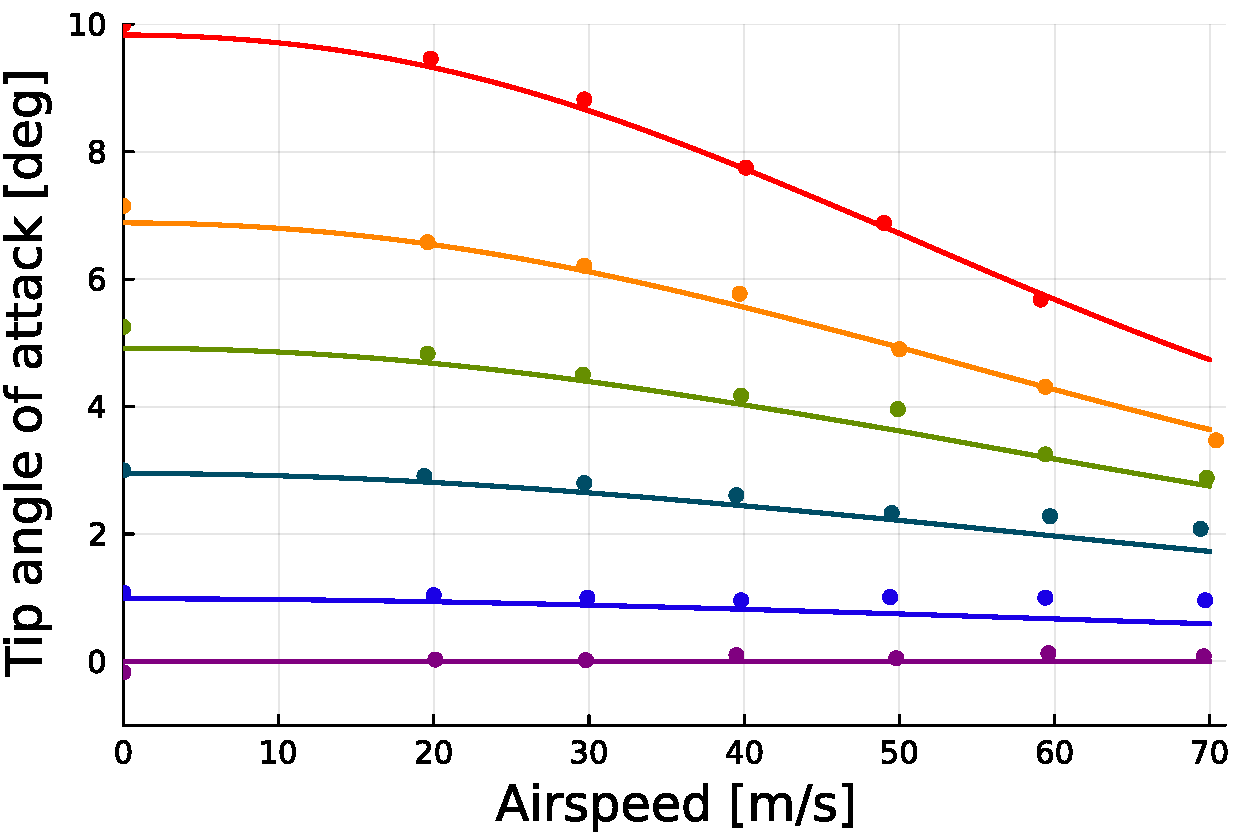
\includegraphics[width=\linewidth]{figures/S10BeamRodSteadyPitchRange_tipAoA.pdf}
        \caption{S10, tip angle of attack.}
        \label{fig:S10BeamRodSteadyPitchRange_tipAoA}
    \end{subfigure}
    \hfill
    \begin{subfigure}[b]{0.48\linewidth}
        \centering
        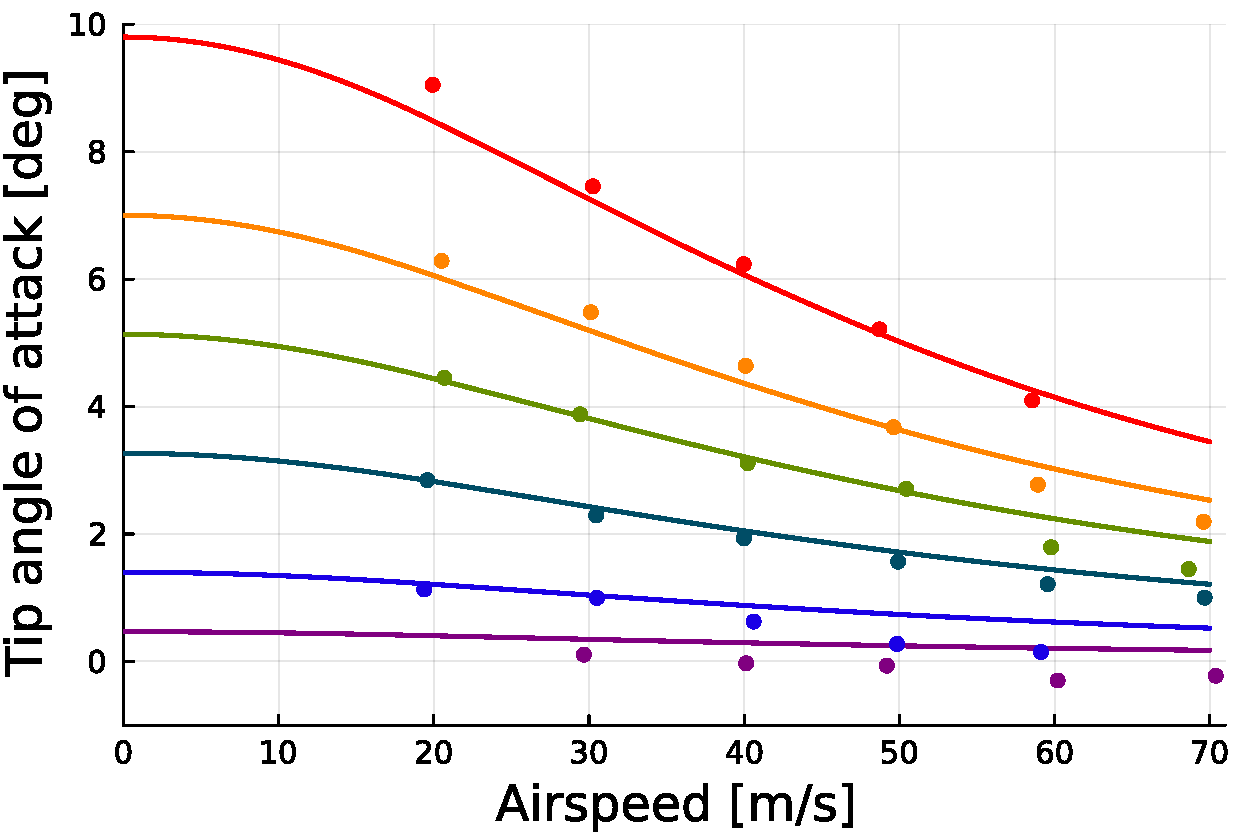
\includegraphics[width=\linewidth]{figures/S20BeamRodSteadyPitchRange_tipAoA.pdf}
        \caption{S20, tip angle of attack.}
        \label{fig:S20BeamRodSteadyPitchRange_tipAoA}
    \end{subfigure}
    \caption{Steady response of the S10 and S20 beam-rod models over the airspeed for the pitch range.}
    \label{fig:S10_S20BeamRodSteadyPitchRange}
\end{figure}

\clearpage

\section{Flutter boundaries}

% S0

\begin{figure}[ht!]
    \centering
    \begin{subfigure}[b]{\textwidth}
        \centering
        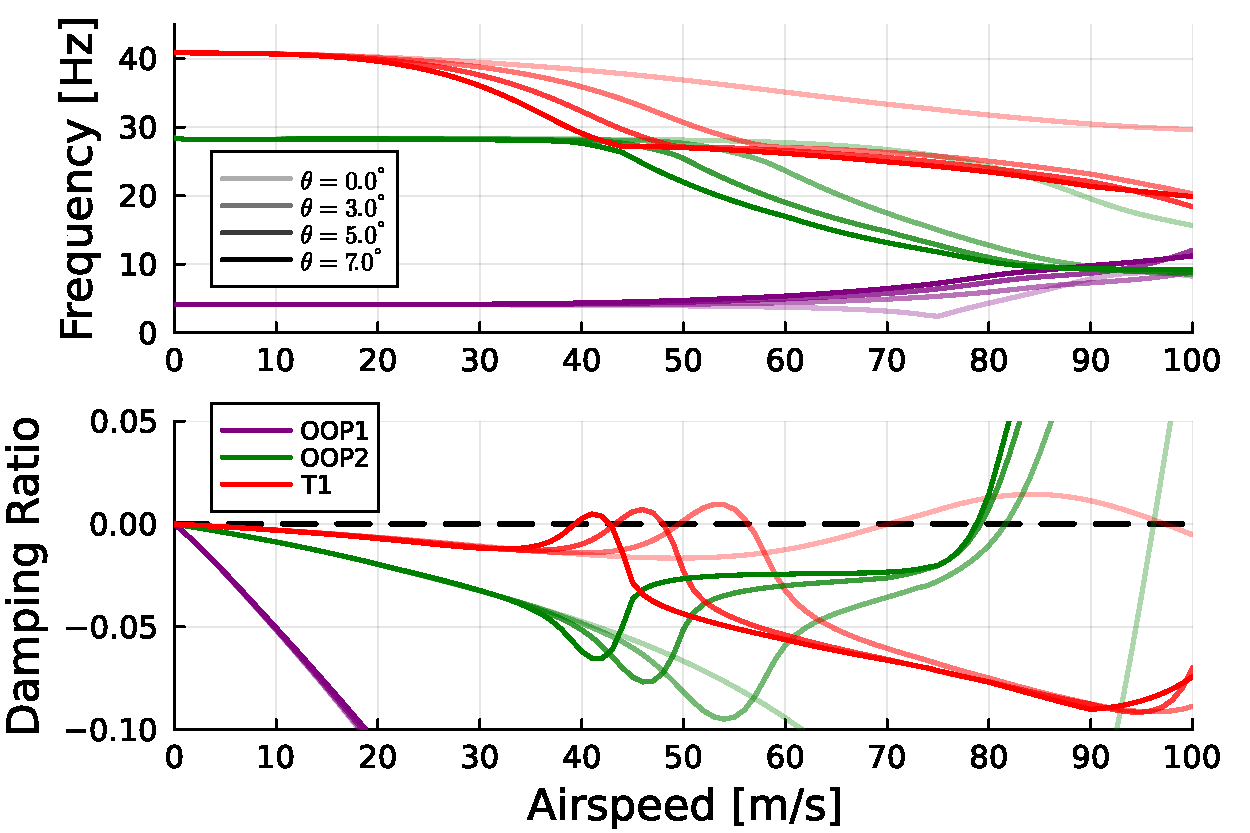
\includegraphics[width=0.7\linewidth]{figures/S0BeamRodFlutterPitchRange_Vgf.pdf}
        \caption{V-g-f over root pitch angle: $\theta=0^\circ,3^\circ,5^\circ,7^\circ$ from lighter to darker colors.}
        \label{fig:S0BeamRodFlutterPitchRange_Vgf}
    \end{subfigure}
    \\[1em]
    \begin{subfigure}[b]{0.495\textwidth}
        \centering
        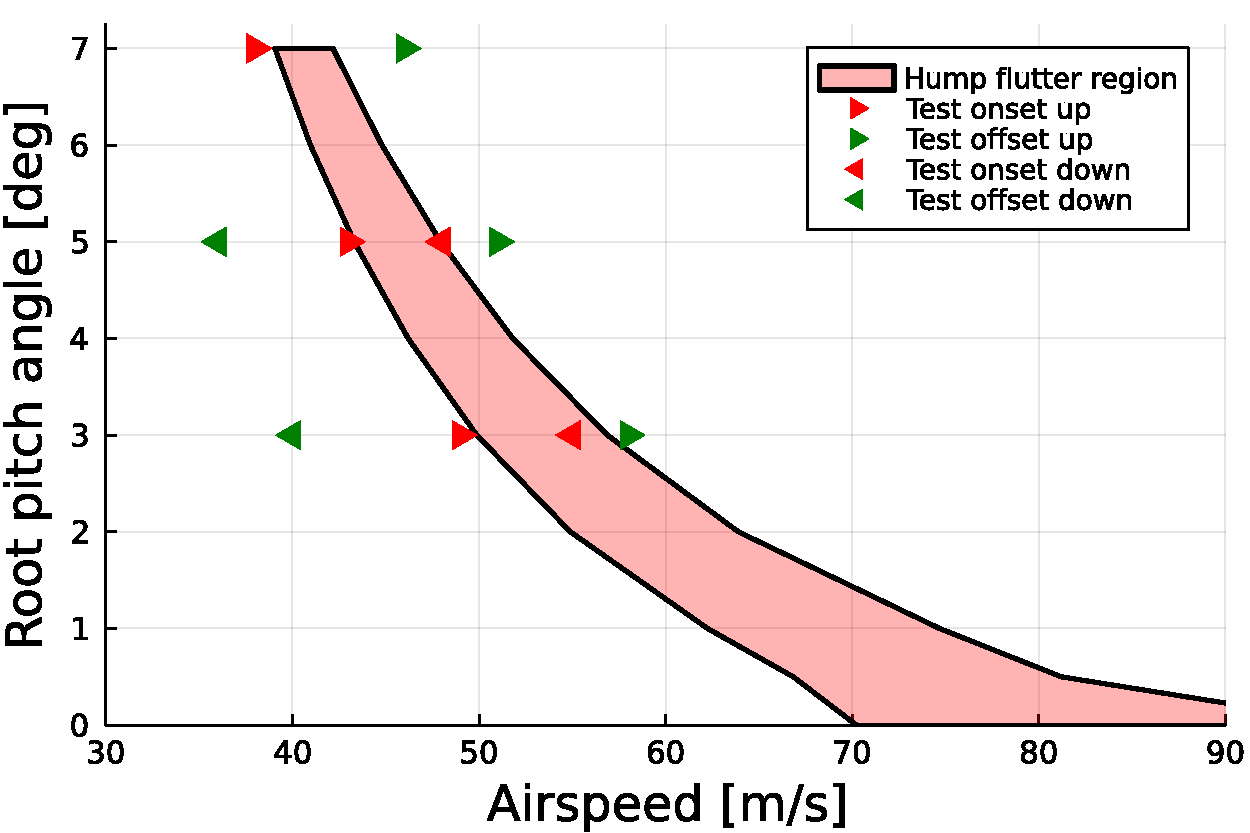
\includegraphics[width=\linewidth]{figures/S0BeamRodHumpFlutterRegion_flutterBoundaryPitch.pdf}
        \caption{Hump flutter boundary (pitch angle effect).}
        \label{fig:S0BeamRodHumpFlutterRegion_flutterBoundaryPitch}
    \end{subfigure}
    \begin{subfigure}[b]{0.495\textwidth}%
        \centering
        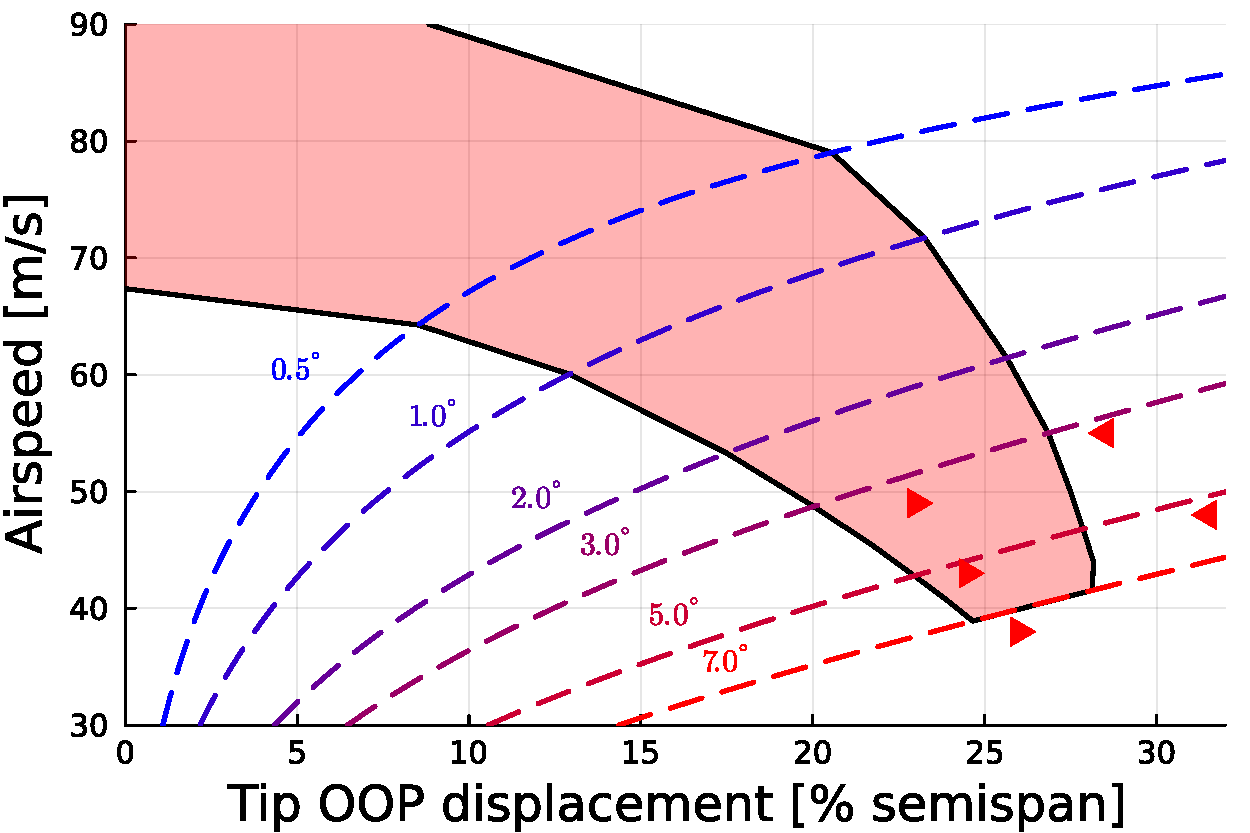
\includegraphics[width=\linewidth]{figures/S0BeamRodHumpFlutterRegion_flutterBoundaryDisp.pdf}
        \caption{Hump flutter boundary (displacement effect).}
        \label{fig:S0BeamRodHumpFlutterRegion_flutterBoundaryDisp}
    \end{subfigure}%
    \caption{S0 beam-rod model: flutter boundary.}
    \label{fig:S0_BeamRod_flutter}
\end{figure}

% S10

\begin{figure}[ht!]
    \centering
    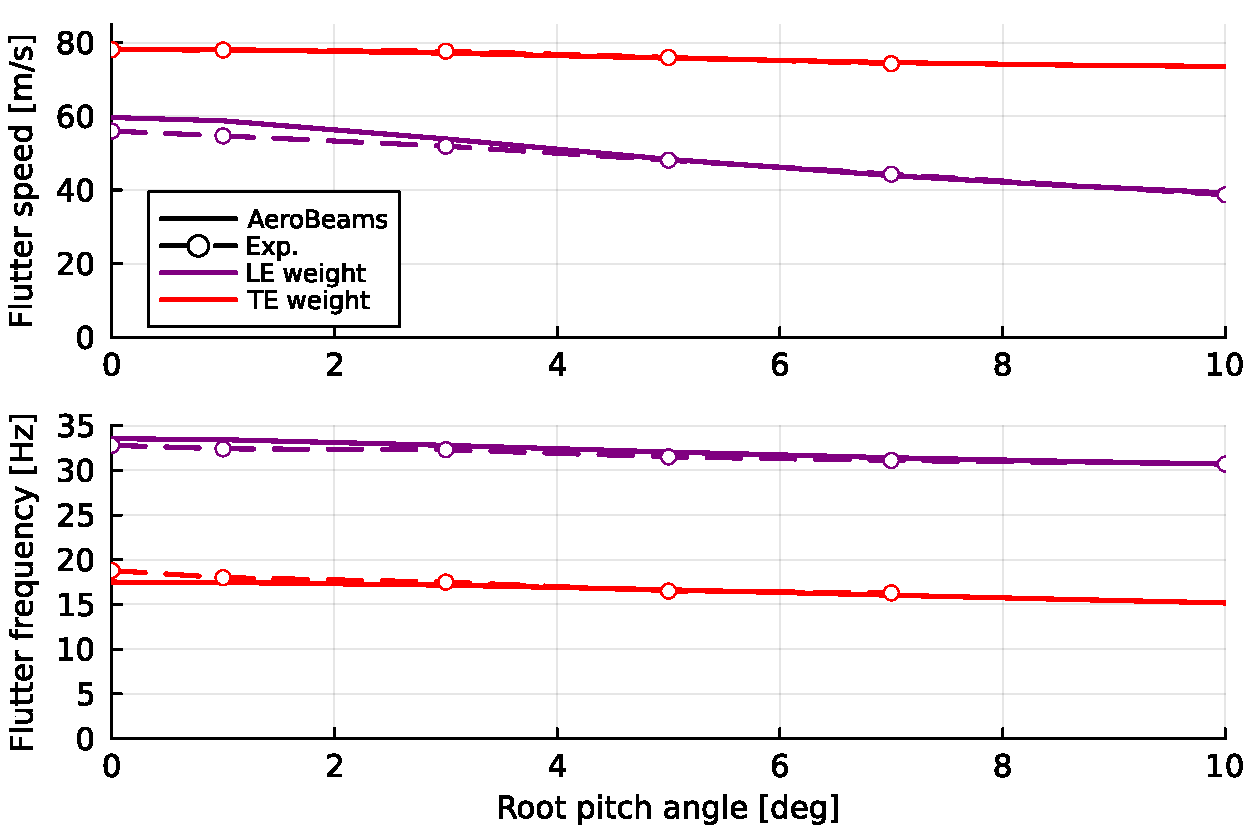
\includegraphics[width=0.8\linewidth]{figures/S10BeamRodFlutterOnsetPitchRange_Uf_omegaf.pdf}
    \caption{S10 beam-rod model: flutter onset airspeed $U_f$ and frequency $\omega_f$ over the pitch range.}
    \label{fig:S10BeamRodFlutterOnsetPitchRange_Uf_omegaf}
\end{figure}

\begin{figure}[ht!]
    \centering
    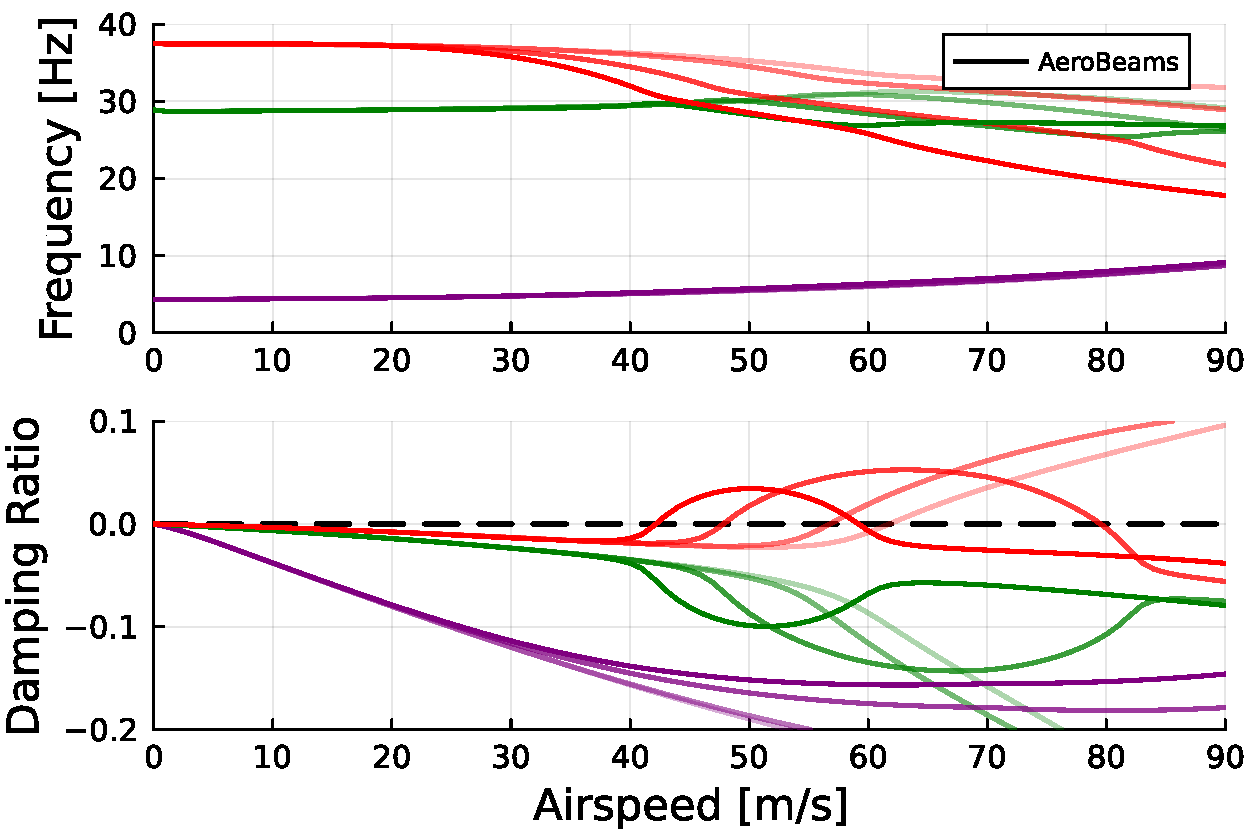
\includegraphics[width=0.8\linewidth]{figures/S10BeamRodFlutterPitchRange_Vgf_LE.pdf}
    \caption{S10 LE beam-rod model: flutter airspeed (V-g) over the pitch range.}
    \label{fig:S10BeamRodFlutterPitchRange_Vgf_LE}
\end{figure}

\begin{figure}[ht!]
    \centering
    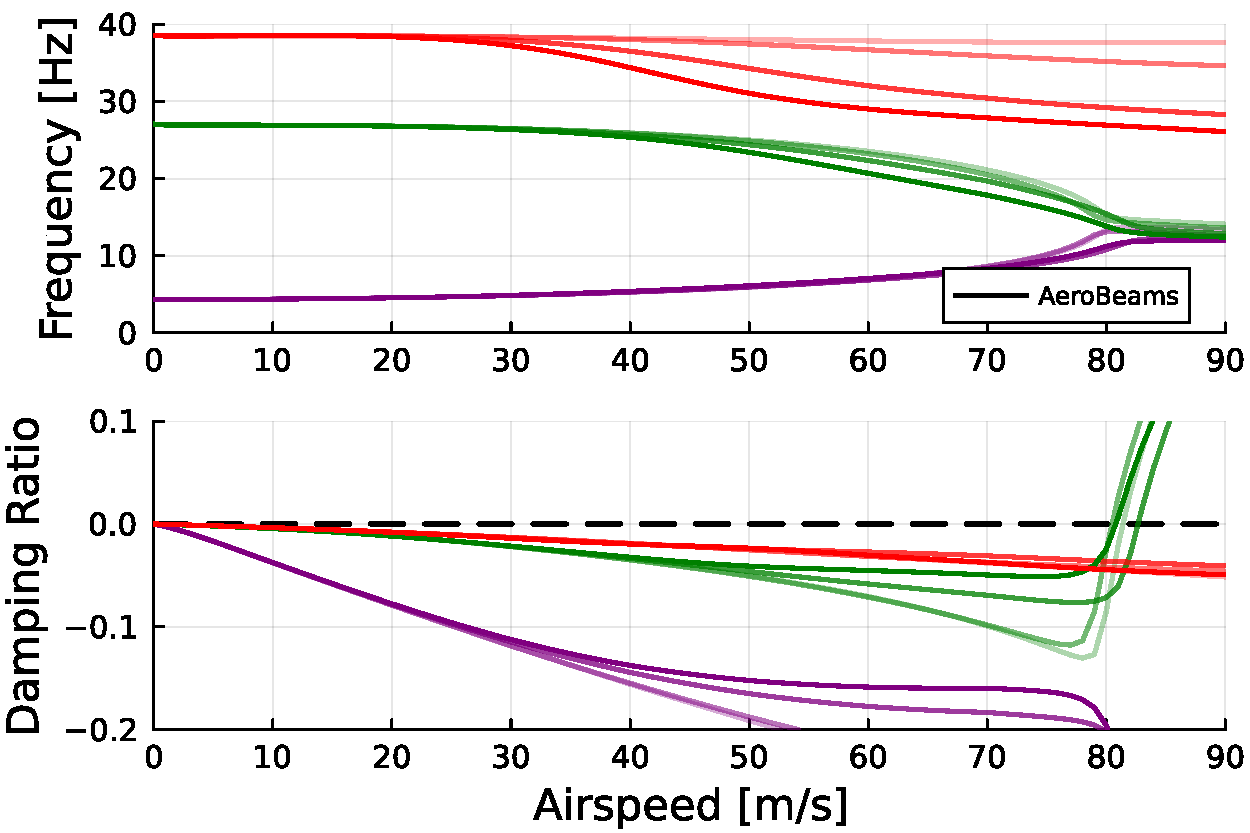
\includegraphics[width=0.8\linewidth]{figures/S10BeamRodFlutterPitchRange_Vgf_TE.pdf}
    \caption{S10 TE beam-rod model: flutter airspeed (V-g) over the pitch range.}
    \label{fig:S10BeamRodFlutterPitchRange_Vgf_TE}
\end{figure}

% S20

\begin{figure}[ht!]
    \centering
    \begin{subfigure}[b]{\textwidth}
        \centering
        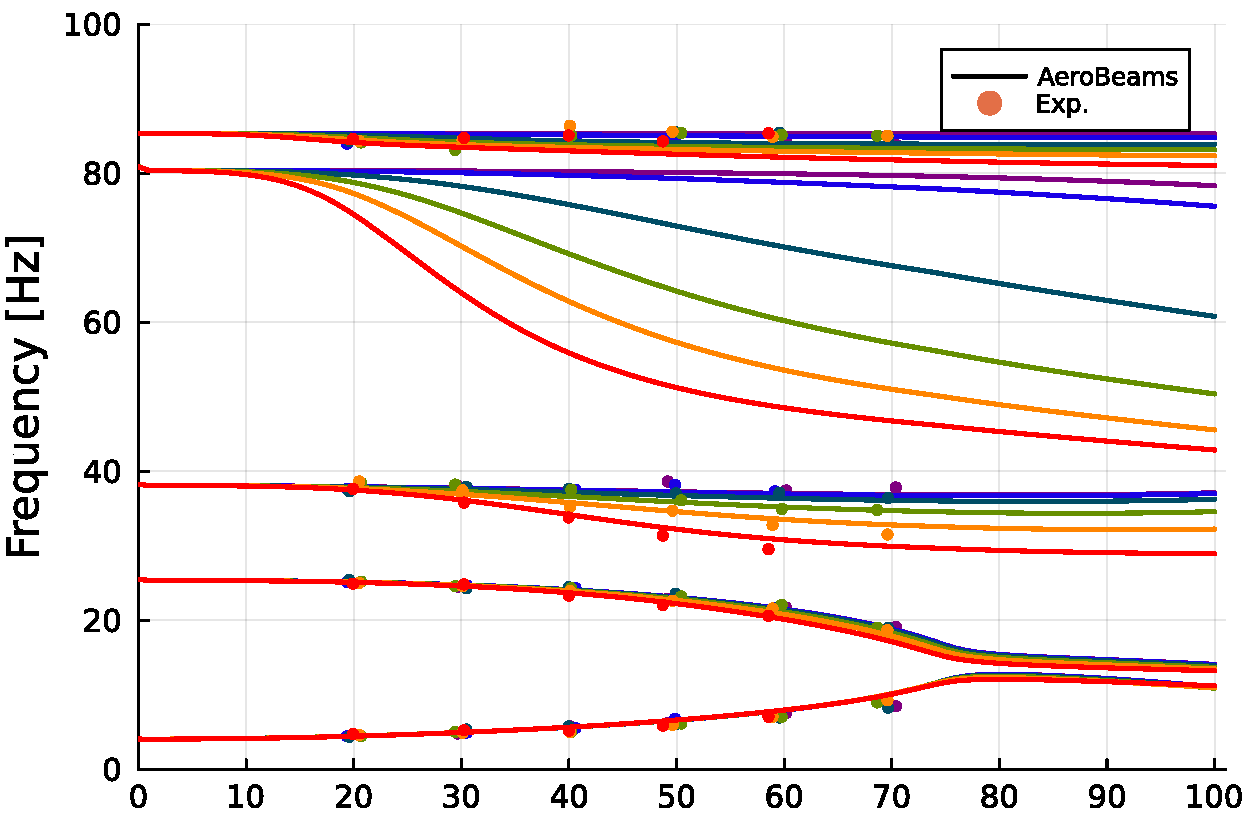
\includegraphics[width=0.7\linewidth]{figures/S20BeamRodFlutterPitchRange_freq_TE.pdf}
        \caption{TE flutter frequency over the pitch range.}
        \label{fig:S20BeamRodFlutterPitchRange_freq_TE}
    \end{subfigure}
    \\[1em]
    \begin{subfigure}[b]{0.495\textwidth}%
        \centering
        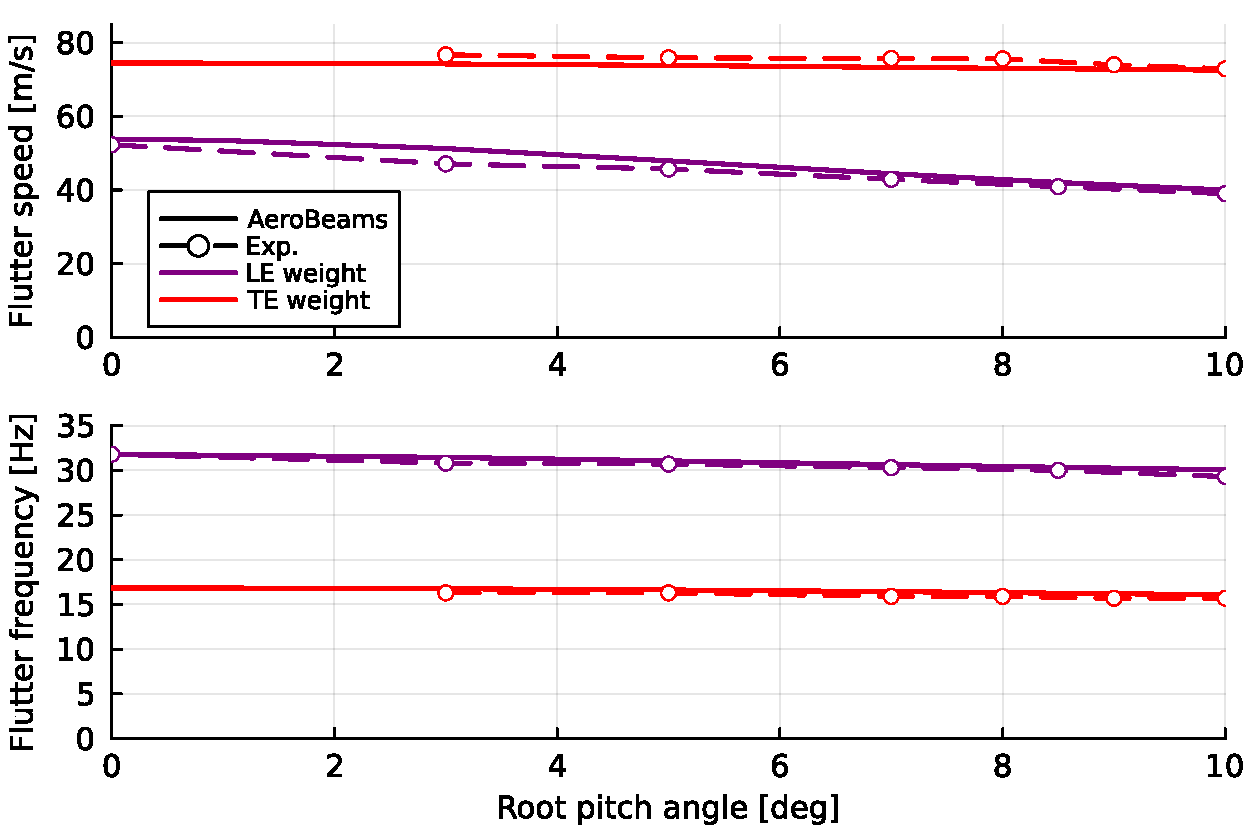
\includegraphics[width=\linewidth]{figures/S20BeamRodFlutterOnsetPitchRange_Uf_omegaf_vs_aoa.pdf}
        \caption{Flutter onset airspeed and frequency versus tip angle of attack.}
        \label{fig:S20BeamRodFlutterOnsetPitchRange_Uf_omegaf_vs_aoa}
    \end{subfigure}%
    \begin{subfigure}[b]{0.495\textwidth}
        \centering
        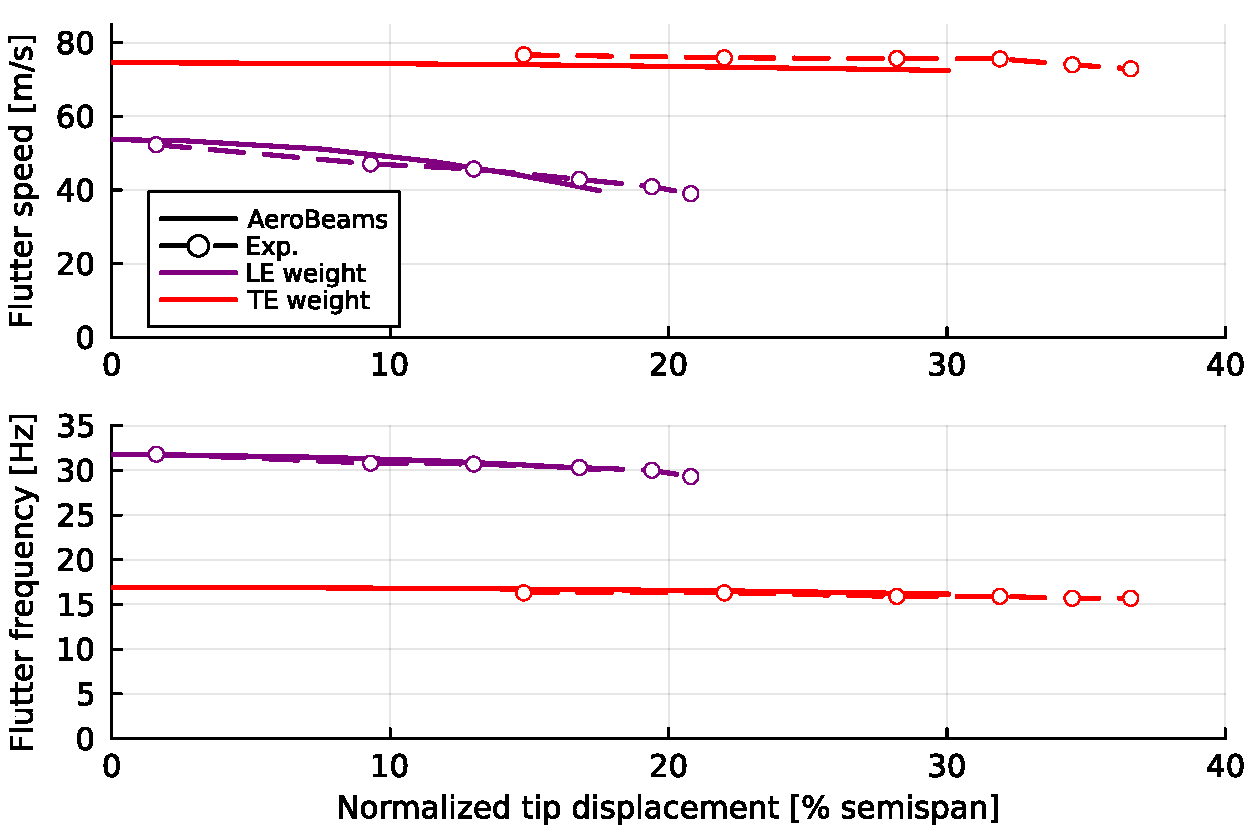
\includegraphics[width=\linewidth]{figures/S20BeamRodFlutterOnsetPitchRange_Uf_omegaf_vs_tipdisp.pdf}
        \caption{Flutter onset airspeed and frequency versus tip displacement.}
        \label{fig:S20BeamRodFlutterOnsetPitchRange_Uf_omegaf_vs_tipdisp}
    \end{subfigure}
    \caption{S20 beam-rod model: flutter results.}
    \label{fig:S20_BeamRod_flutter}
\end{figure}

\clearpage

\section{Limit-cycle oscillations}
\label{sec:limit_cycle_oscillations}

% S10 inertia rod

\begin{figure}[ht!]
    \centering
    \begin{subfigure}[b]{0.7\textwidth}
        \centering
        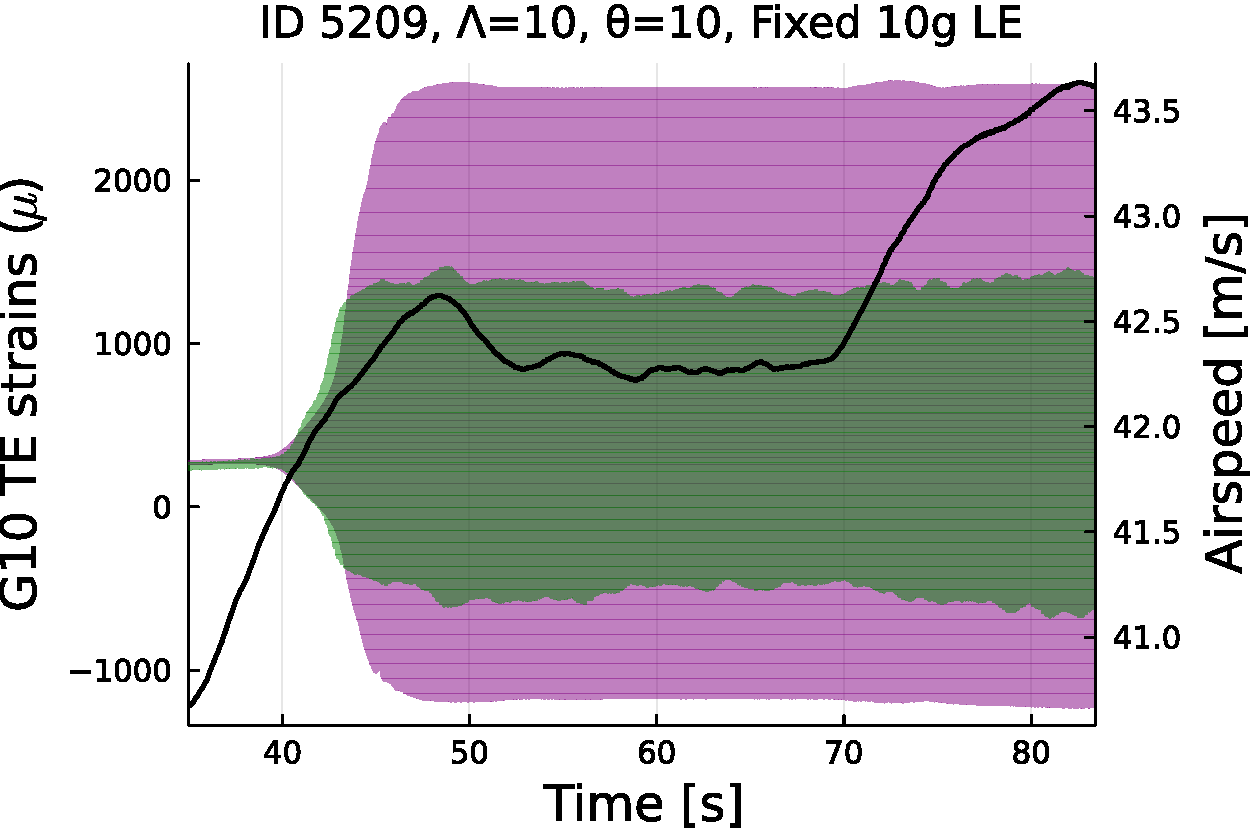
\includegraphics[width=\linewidth]{figures/S10InertiaRodMatchingAirspeedSweep_ID5209_VLM-def_Indicial_g10EpsTE.pdf}
        \caption{TE strain time history at 60\% span.}
        \label{fig:S10InertiaRodMatchingAirspeedSweep_ID5209_VLM-def_Indicial_g10EpsTE}
    \end{subfigure}
    \\[1em]
    \begin{subfigure}[b]{0.495\textwidth}%
        \centering
        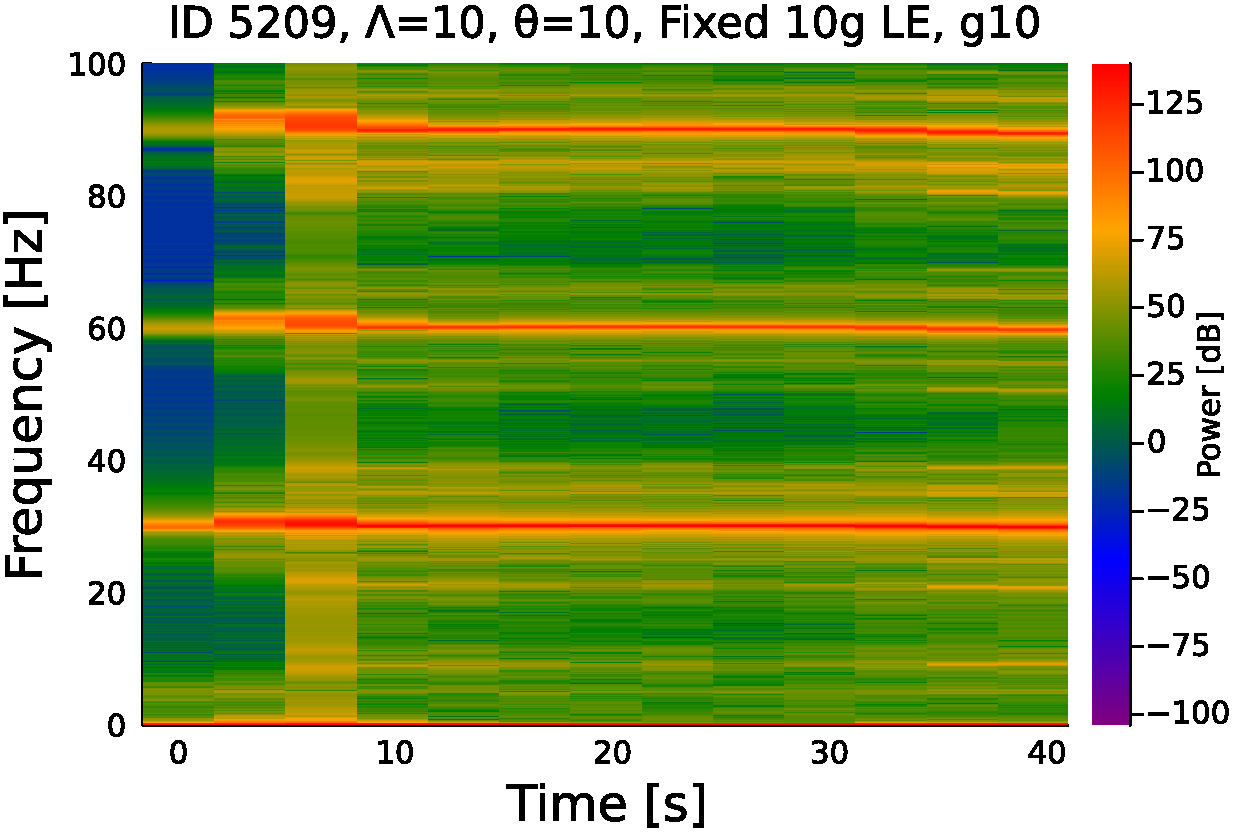
\includegraphics[width=\linewidth]{figures/S10InertiaRodMatchingAirspeedSweep_ID5209_VLM-def_Indicial_g10EpsTESpectrogram.pdf}
        \caption{TE strain spectrogram at 60\% span.}
        \label{fig:S10InertiaRodMatchingAirspeedSweep_ID5209_VLM-def_Indicial_g10EpsTESpectrogram}
    \end{subfigure}%
    \begin{subfigure}[b]{0.495\textwidth}
        \centering
        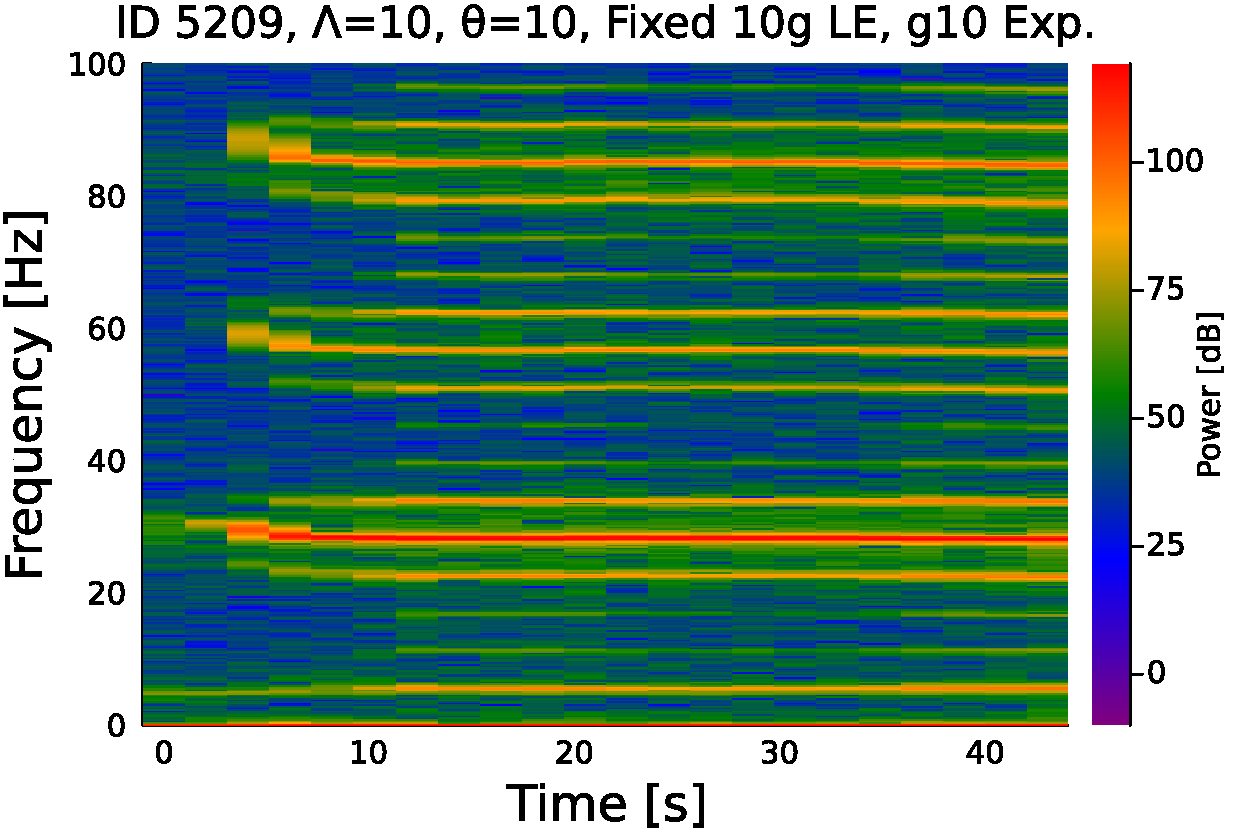
\includegraphics[width=\linewidth]{figures/ID5209_g10EpsTESpectrogram_exp.pdf}
        \caption{Experimental TE strain spectrogram at 60\% span.}
        \label{fig:ID5209_g10EpsTESpectrogram_exp}
    \end{subfigure}
    \caption{S10 inertia-rod matching airspeed sweep (ID 5209, VLM-def, indicial).}
    \label{fig:S10_inertia_rod_matching_g10}
\end{figure}

% S10 beam rod

\begin{figure}[ht!]
    \centering
    \begin{subfigure}[b]{0.7\textwidth}%
        \centering
        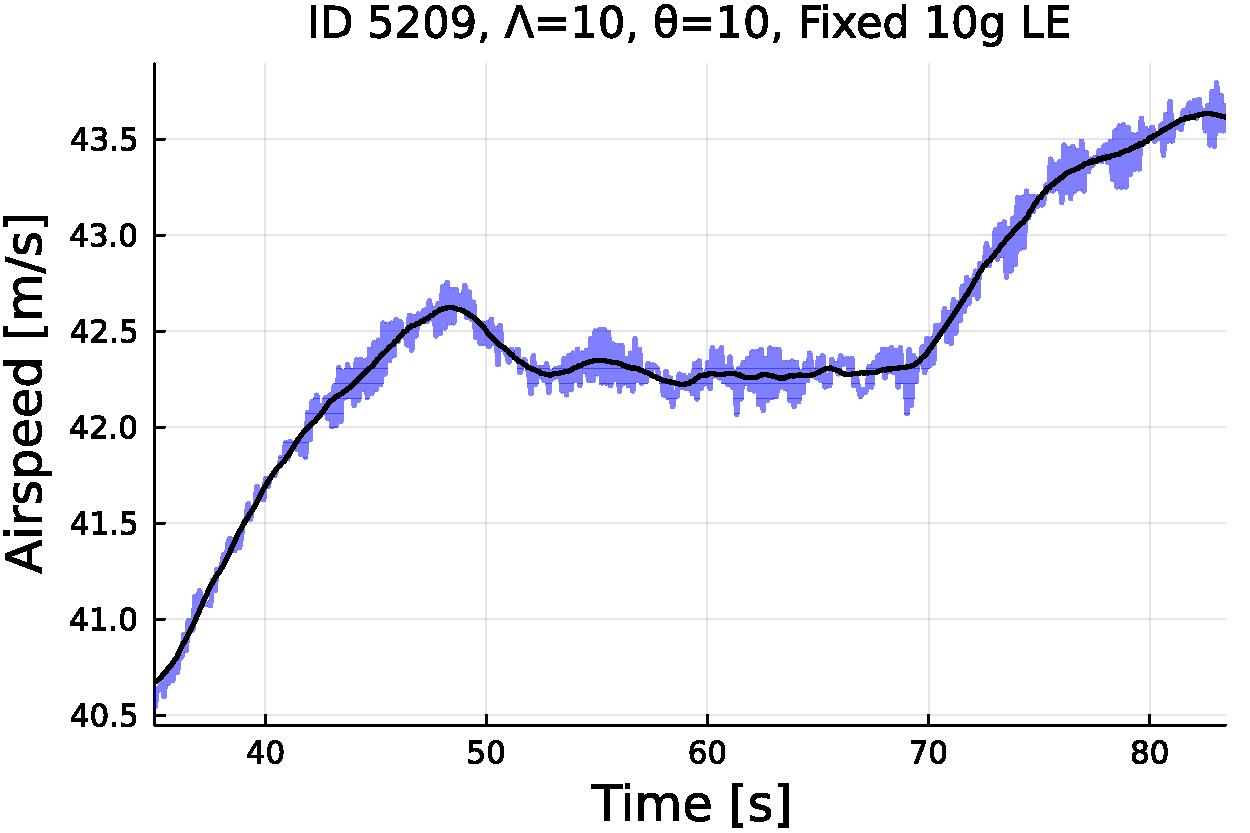
\includegraphics[width=\linewidth]{figures/S10BeamRodMatchingAirspeedSweep_ID5209_VLM-def_Indicial_U.pdf}
        \caption{Airspeed profile.}
        \label{fig:S10BeamRodMatchingAirspeedSweep_ID5209_VLM-def_Indicial_U}
    \end{subfigure}%
    \\[1em]
    \begin{subfigure}[b]{0.495\textwidth}
        \centering
        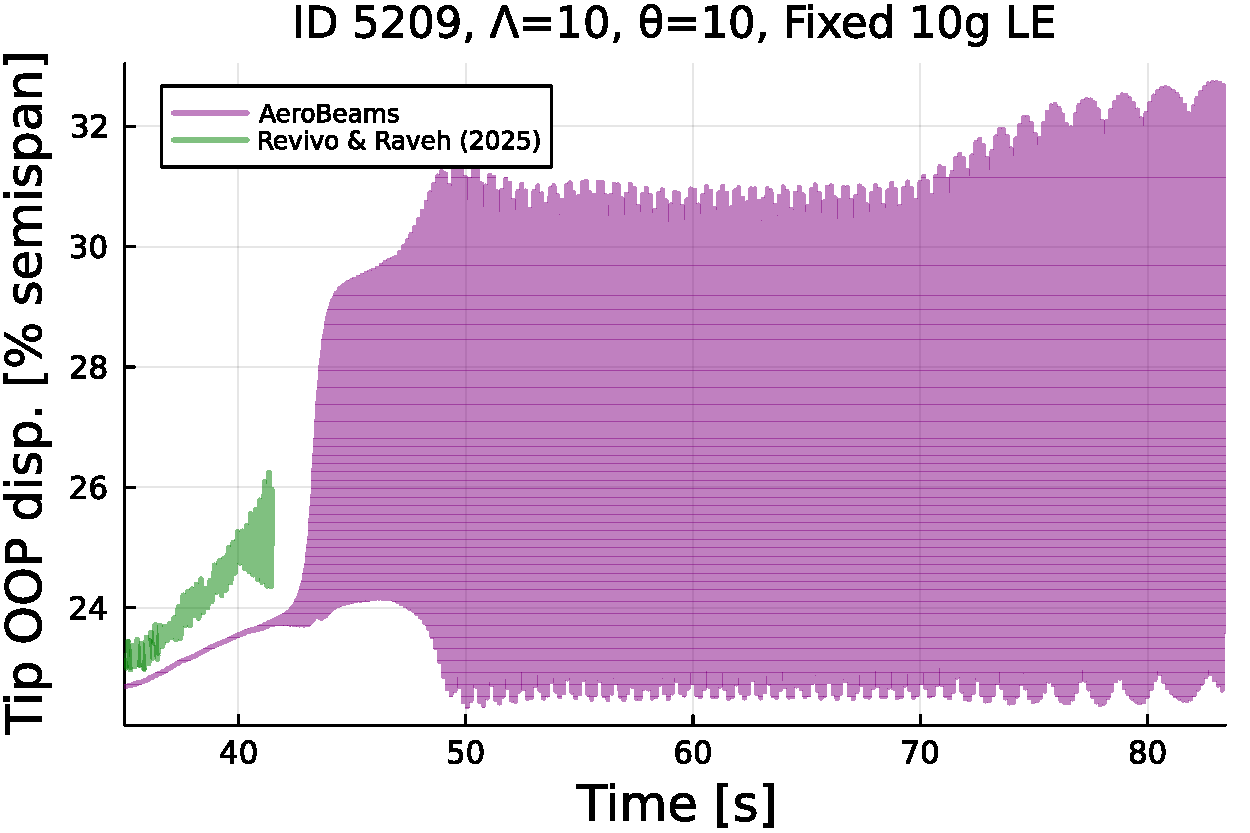
\includegraphics[width=\linewidth]{figures/S10BeamRodMatchingAirspeedSweep_ID5209_VLM-def_Indicial_tipOOP.pdf}
        \caption{Tip out-of-plane displacement.}
        \label{fig:S10BeamRodMatchingAirspeedSweep_ID5209_VLM-def_Indicial_tipOOP}
    \end{subfigure}
    \begin{subfigure}[b]{0.495\textwidth}%
        \centering
        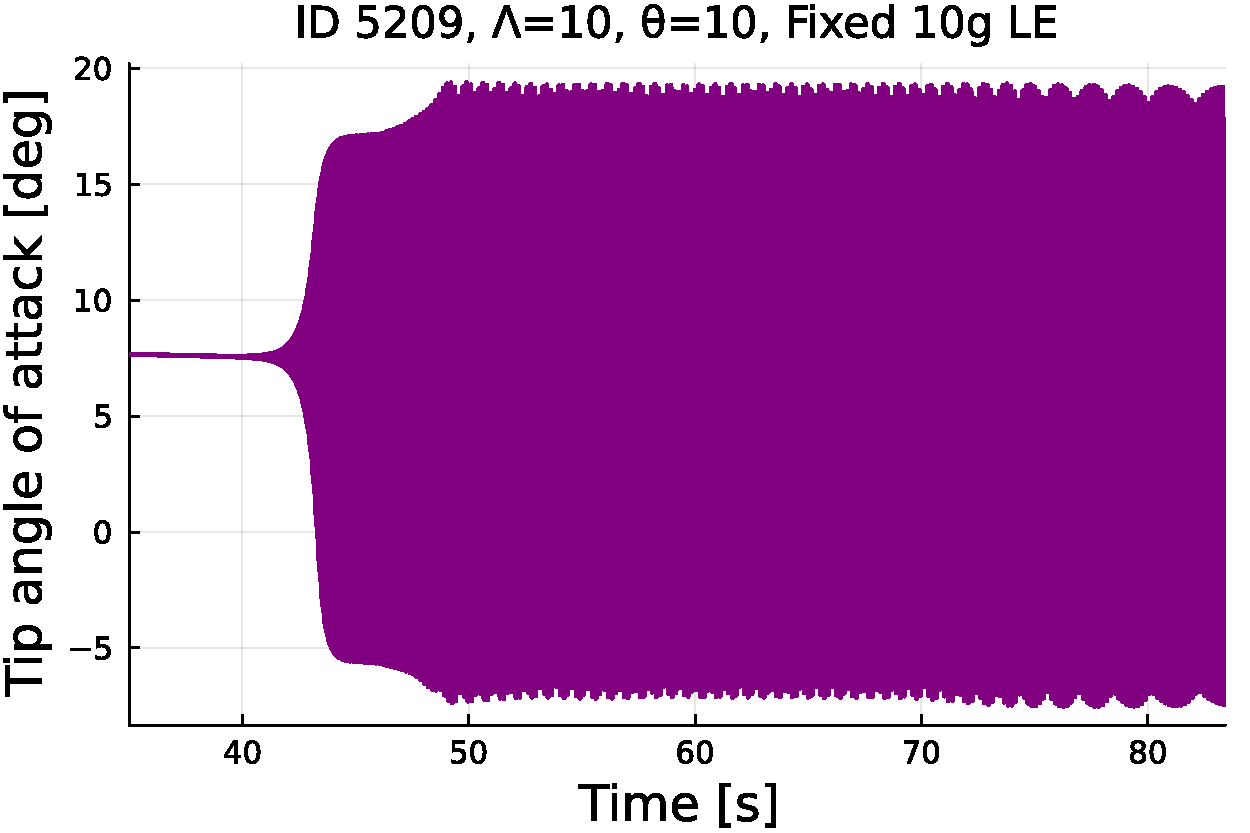
\includegraphics[width=\linewidth]{figures/S10BeamRodMatchingAirspeedSweep_ID5209_VLM-def_Indicial_tipAoA.pdf}
        \caption{Tip angle of attack.}
        \label{fig:S10BeamRodMatchingAirspeedSweep_ID5209_VLM-def_Indicial_tipAoA}
    \end{subfigure}%
    \\[1em]
    \begin{subfigure}[b]{0.495\textwidth}%
        \centering
        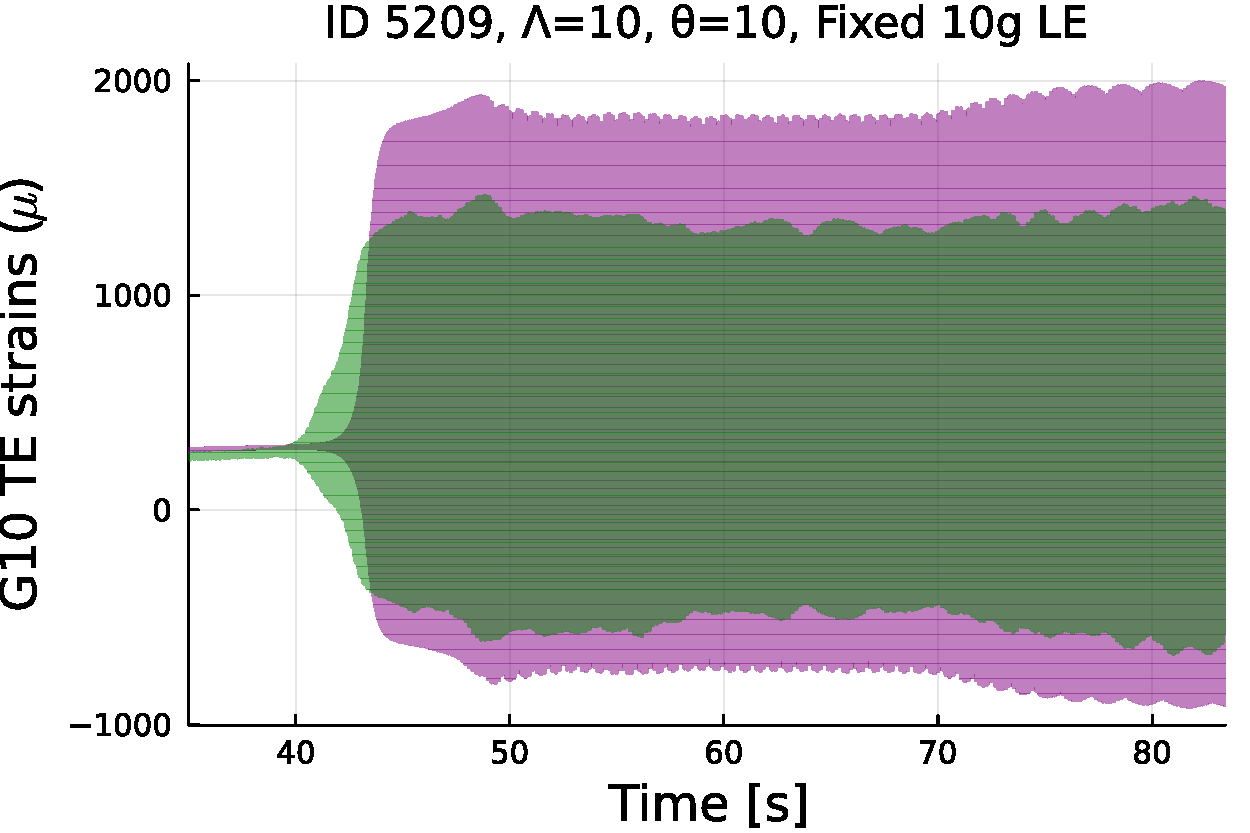
\includegraphics[width=\linewidth]{figures/S10BeamRodMatchingAirspeedSweep_ID5209_VLM-def_Indicial_g10EpsTE.pdf}
        \caption{TE strain at 60\% span.}
        \label{fig:S10BeamRodMatchingAirspeedSweep_ID5209_VLM-def_Indicial_g10EpsTE}
    \end{subfigure}%
    \begin{subfigure}[b]{0.495\textwidth}
        \centering
        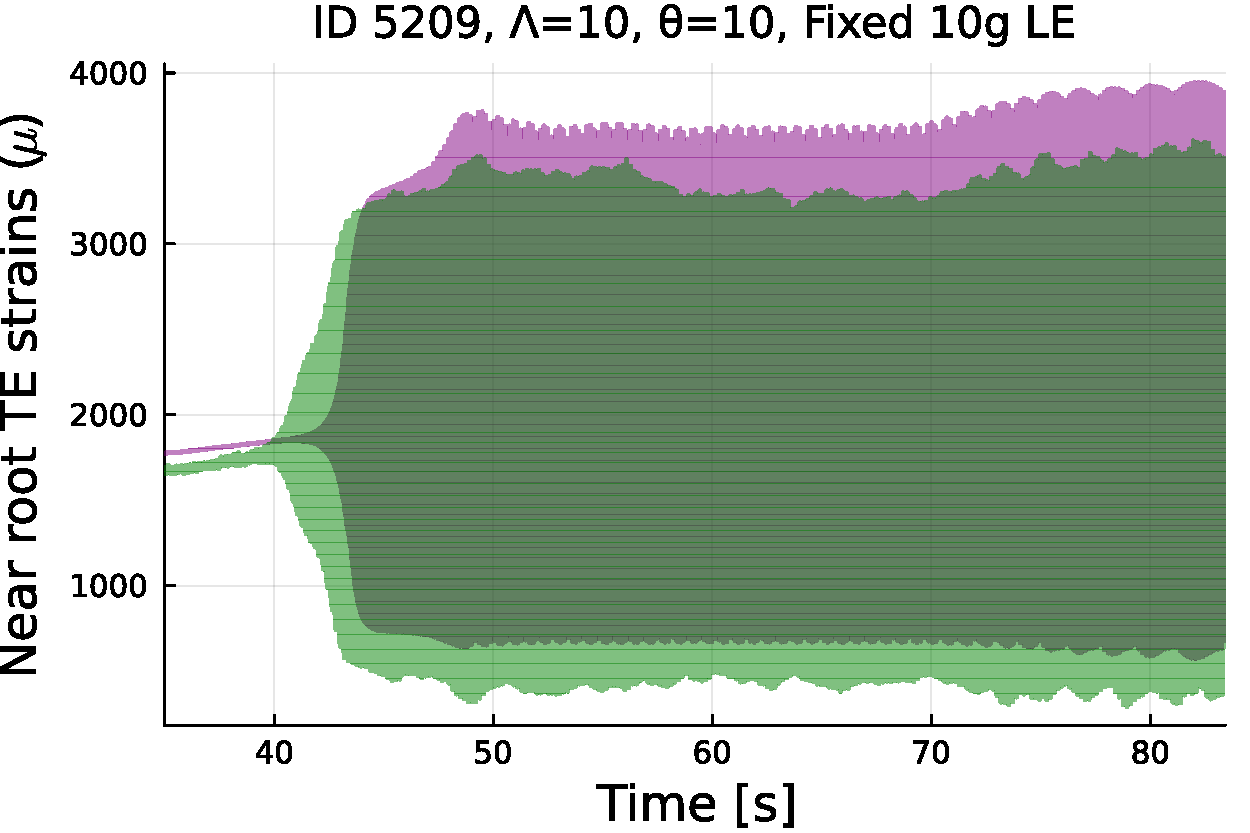
\includegraphics[width=\linewidth]{figures/S10BeamRodMatchingAirspeedSweep_ID5209_VLM-def_Indicial_rootEpsTE.pdf}
        \caption{Near-root TE strain.}
        \label{fig:S10BeamRodMatchingAirspeedSweep_ID5209_VLM-def_Indicial_rootEpsTE}
    \end{subfigure}
    \caption{S10 beam-rod LCO (ID 5209, VLM-def, indicial).}
    \label{fig:S10_beamrod_ID5209_LCO}
\end{figure}

\begin{figure}
    \centering
    \begin{subfigure}[b]{0.7\textwidth}
        \centering
        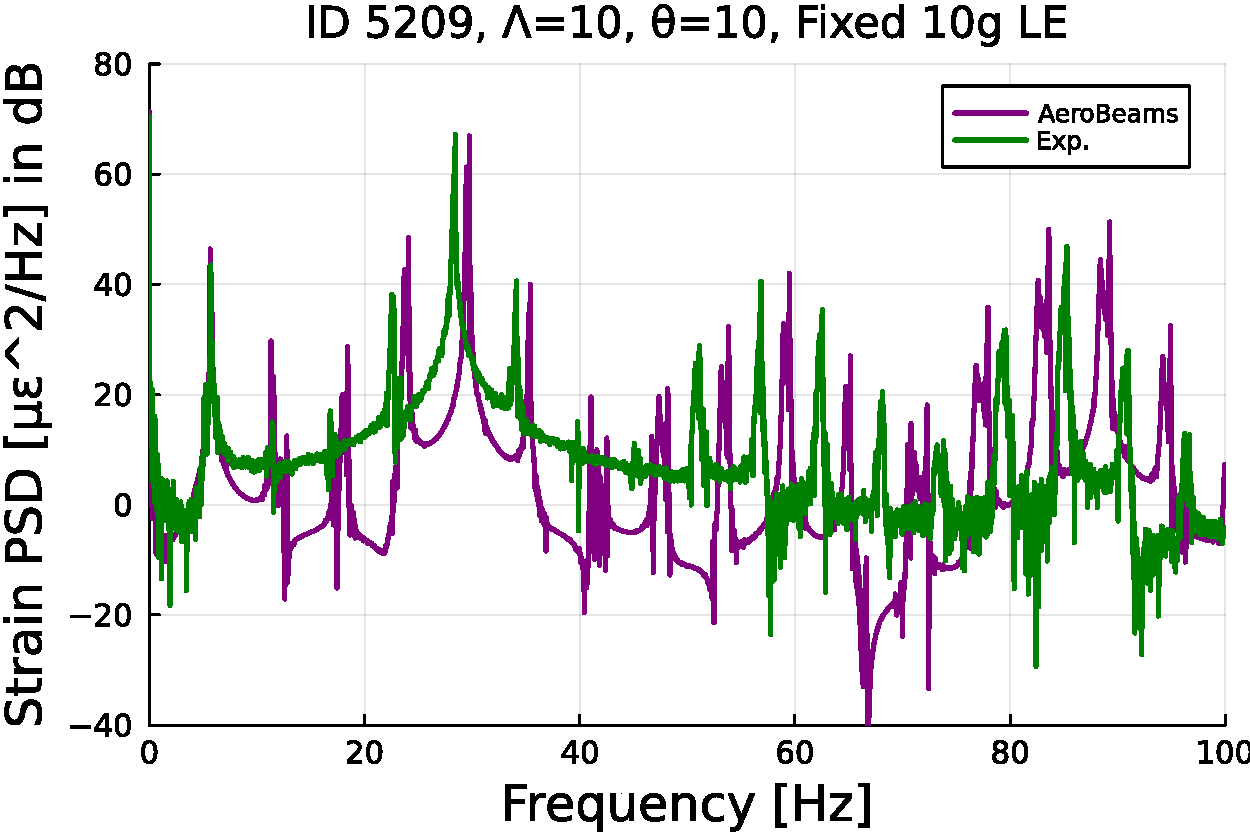
\includegraphics[width=\linewidth]{figures/S10BeamRodMatchingAirspeedSweep_ID5209_VLM-def_Indicial_g10EpsTEPSD.pdf}
        \caption{TE strain PSD at 60\% span.}
        \label{fig:S10BeamRodMatchingAirspeedSweep_ID5209_VLM-def_Indicial_g10EpsTEPSD}
    \end{subfigure}
    \\[1em]
    \begin{subfigure}[b]{0.495\textwidth}%
        \centering
        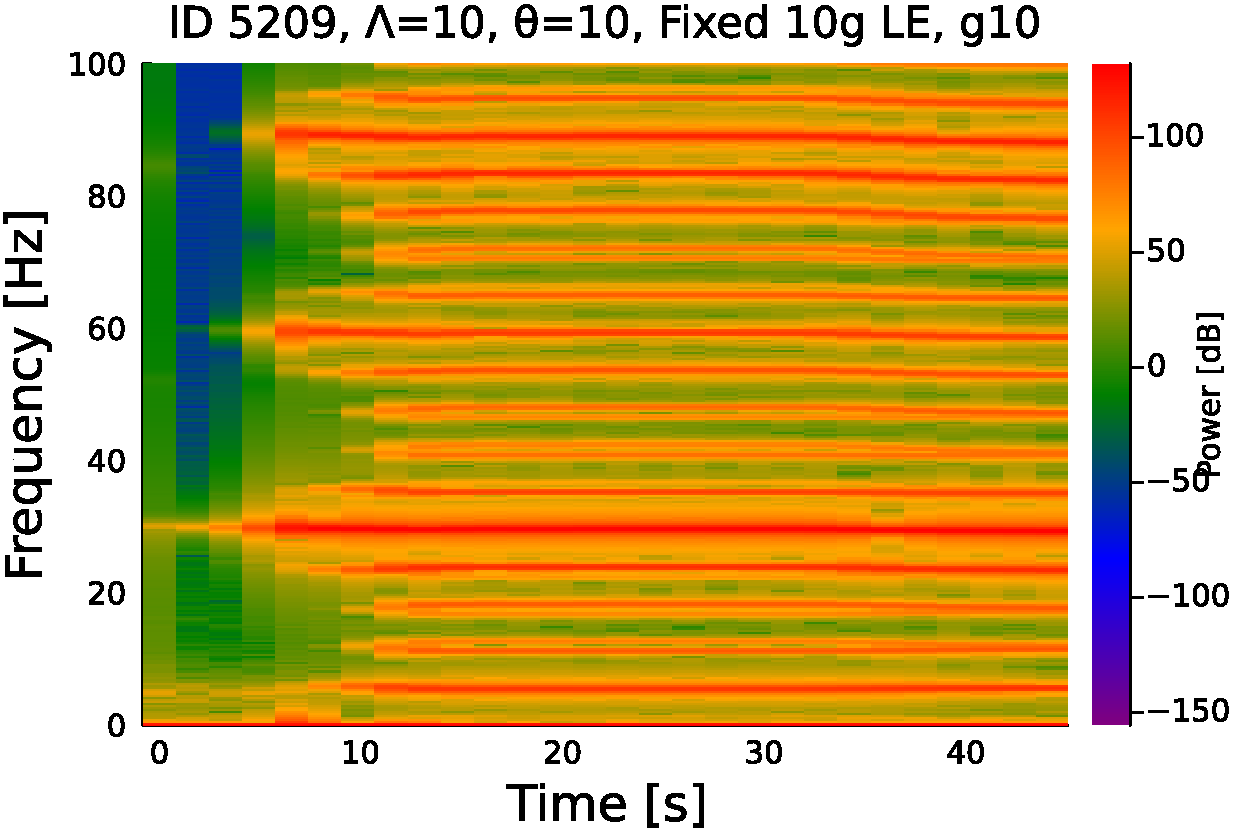
\includegraphics[width=\linewidth]{figures/S10BeamRodMatchingAirspeedSweep_ID5209_VLM-def_Indicial_g10EpsTESpectrogram.pdf}
        \caption{TE strain spectrogram at 60\% span.}
        \label{fig:S10BeamRodMatchingAirspeedSweep_ID5209_VLM-def_Indicial_g10EpsTESpectrogram}
    \end{subfigure}%
    \begin{subfigure}[b]{0.495\textwidth}%
        \centering
        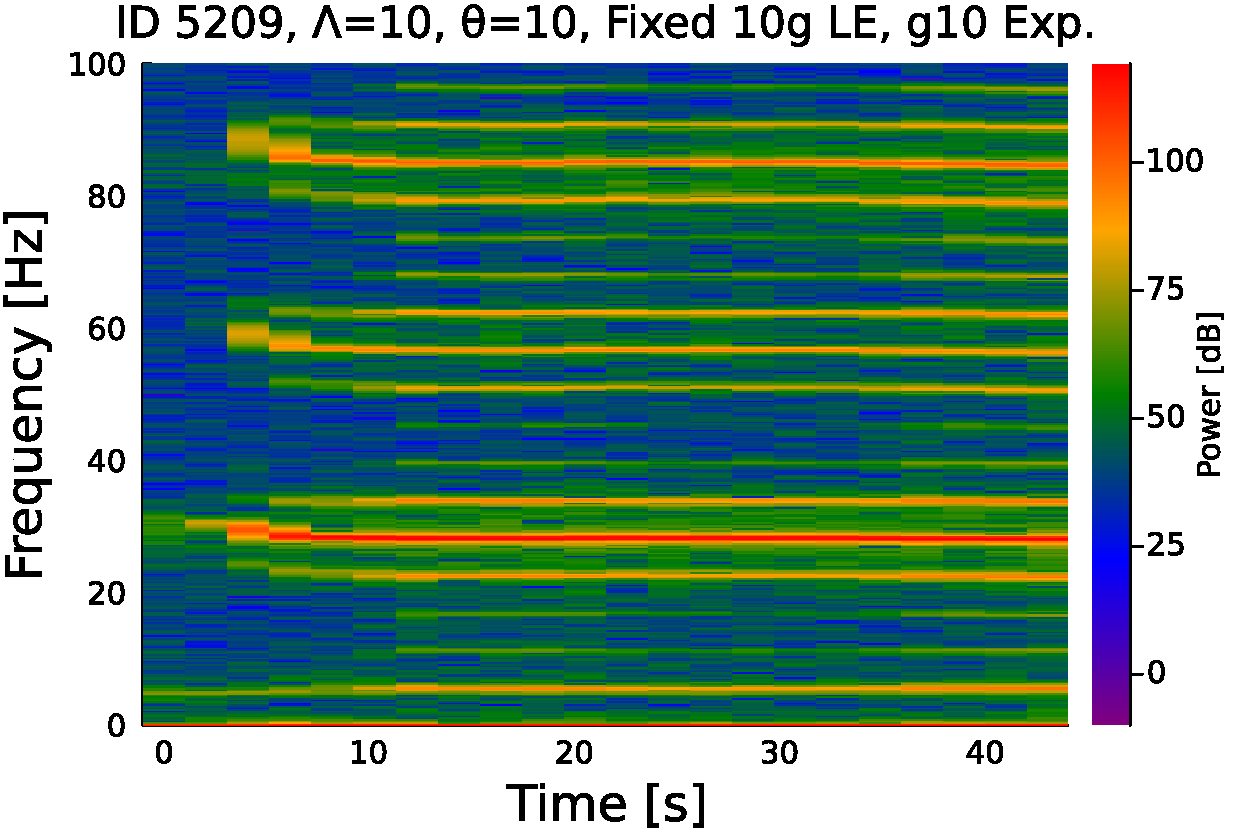
\includegraphics[width=\linewidth]{figures/ID5209_g10EpsTESpectrogram_exp.pdf}
        \caption{TE strain spectrogram at 60\% span (exp.).}
        \label{fig:ID5209_g10EpsTESpectrogram_exp2}
    \end{subfigure}
    \caption{S10 beam-rod spectrogram (ID 5209, VLM-def, indicial).}
    \label{fig:S10_beamrod_ID5209_spectrogram}
\end{figure}

\section{Conclusion}


\section*{Acknowledgments}
The authors acknowledge the support of the S\~ao Paulo Research Foundation (FAPESP), grants $\#$2025/17343-5 and $\#$2022/13836-9 and the Brazilian National Council for Scientific and Technological Development – CNPq, Brazil, grant $\#$306824/2019-1.

\bibliography{references}

\clearpage

\appendix
\section{Beam condensation from generalized finite element models}
\label{sec:beam_condensation}

The Pazy (in its S0, S10 and S20 variants) is a complex built-up structure, composed of an aluminum spar, a 3-D printed chassis (ribs, leading- and trailing-edge stringers, and wingtip rod, all made of Nylon), and a thin polyester skin that gives the wing its aerodynamic contour. The wingtip rod and weights attached to it are an essential part of tuning the dynamic response of the wing, significantly affecting its modal characteristics. The large (Nastran) finite element models also include calibration masses and the instrumentation, such as cabling, strain gauges, etc., necessary for experimental validation, which are present in the physical setup as shown in \cref{fig:Pazy_models}.

\begin{figure}[ht!]
    \begin{center}
        \centering		
        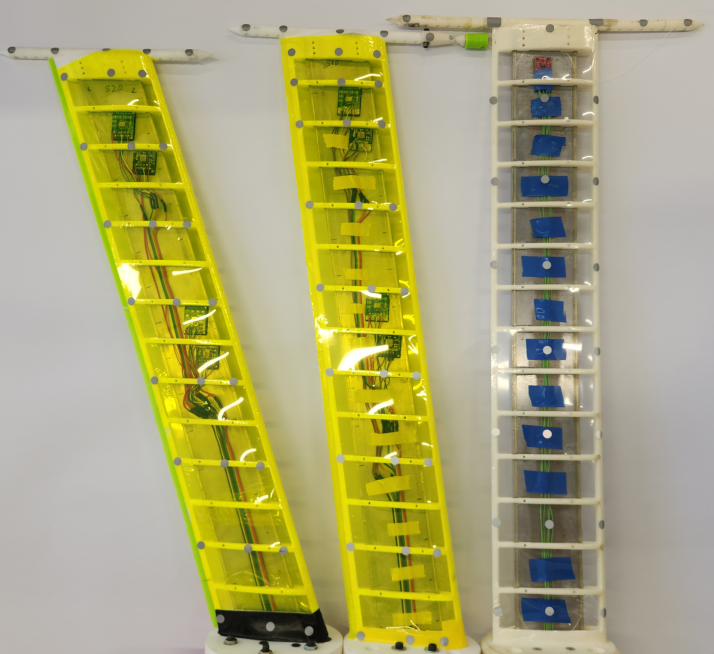
\includegraphics[width=0.8\linewidth,trim={0cm 0cm 0cm 0cm}, clip]{figures/Pazy_models.png}
        \caption{Straight (S0, on the right), and swept (S10 in the middle and S20 on the left) configurations of the Pazy. Courtesy of Technion.}
        \label{fig:Pazy_models}
	\end{center}
\end{figure}

Traditional cross-sectional analysis tools, such as \begin{small}VABS\end{small} \cite{hodges2006nonlinear}, produce theoretically grounded and accurate results for smoothly varying cross-sections, but are not sufficient to capture the discretely spanwise-varying properties of the Pazy. Therefore, an alternative approach based on the condensation of generalized finite element models (GFEMs) into a beam model was developed and adopted, called BeamROM. Two modules are necessary to fully characterize the structural behavior: one for the inertial properties and another for the stiffness properties. In both, the student version of Simcenter Femap's Nastran solver was used to perform the necessary finite element analyses on the GFEM.

On the inertial side, an approach analogous to that of \cite{riso2022low} is employed, in which the mass of each of the GFEM's nodes is condensed into the spanwise closest node of a user-defined reference axis of the beam. Each two consecutive nodes of this axis define a beam finite element. Suppose the GFEM has $N$ nodes with lumped masses $m_i$, located at positions $\vect{r}_i$ (the node's position plus the offset of its lumped mass), and lumped inertia tensors $\tens{J}_i$ about $\vect{r}_i$, $i=1,\dots,N$, all in the GFEM's global reference frame. Let the beam nodes be at positions $\vect{x}_k$, $k=1,\dots,K$, and let $\mathcal{L}_k$ be the set of GFEM nodes assigned to beam node $k$, i.e., those whose coordinate along the reference axis' direction is closest to that of $\vect{x}_k$. A GFEM node exactly midway between two consecutive beam nodes belongs to both of their sets, and its mass and inertia are split equally between them. This is accounted for by the weight $w_i$, equal to $1/2$ for such nodes and to $1$ otherwise, such that the total mass is preserved. Then, the equivalent lumped mass of beam node $k$, the offset of its center of mass from the node, and the inertia tensor about the center of mass are
\begin{align}
    m_k &= \sum_{i \in \mathcal{L}_k} w_i m_i \ \ ,
    \\
    \vect{\delta}_k &= \frac{1}{m_k} \sum_{i \in \mathcal{L}_k} w_i m_i \vect{r}_i - \vect{x}_k \ \ ,
    \\
    \tens{J}_k &= \sum_{i \in \mathcal{L}_k} w_i \left[ \tens{J}_i + m_i \lp \norm{\vect{d}_i}^2 \tens{I}_3 - \vect{d}_i \vect{d}_i^\top \rp \right] \ \ , \quad \vect{d}_i = \vect{r}_i - \vect{x}_k - \vect{\delta}_k \ \ ,
\end{align}
where $\tens{I}_3$ is the $3\times 3$ identity matrix. When read by AeroBeams, these tensorial quantities are transformed to the beam's local reference frame, and are used to construct the sectional inertia matrix $\Mass_e$ for each beam element $e$ taking half of the contributions from its nodes $k$ and $k+1$ (except for the first and last elements, which take the full contribution from their respective end nodes).

On the stiffness side, the condensation is performed exploiting a closed-form solution for the linear static tip generalized displacements of a cantilevered beam given the loads applied at its free end, applicable to prismatic beams of composite cross-section. As shown by Hodges \cite{hodges2006nonlinear}, the tip displacements $\hat{\u}$ and rotation angles $\hat{\vect{\theta}}$ of such a cantilevered beam can be expressed in terms of the applied tip forces $\hat{\vect{F}}$ and moments $\hat{\vect{M}}$ as
\begin{align}
    \begin{bmatrix}
        \hat{\u} \\
        \hat{\vect{\theta}}
    \end{bmatrix}
    =
    \underbrace{
    \begin{bmatrix}
        \ell\tens{D} + \dfrac{\ell^2}{2} \lp\tens{Z}\aonetil-\aonetil\tens{Z}^\T\rp - \dfrac{\ell^3}{3}\aonetil\tens{T}\aonetil & \ell\tens{Z} - \dfrac{\ell^2}{2}\aonetil\tens{T} \\
        \ell\tens{Z}^\T + \dfrac{\ell^2}{2}\tens{T}\aonetil & \ell\tens{T}
    \end{bmatrix}
    }_{\large\tens{\mathcal{C}_\text{global}}}
    \begin{bmatrix}
        \hat{\vect{F}} \\
        \hat{\vect{M}}
    \end{bmatrix} \ \ ,
\end{align}
as long as the response is kept within the geometrically linear regime, that is, the displacements and rotations remain small. In this equation, $\ell$ is the length of the beam, $\tens{\mathcal{C}_\text{global}}$ represents a global flexibility matrix, and $\tens{D}$, $\tens{Z}$, and $\tens{T}$ are components of the beam's sectional compliance matrix, i.e,
\begin{align}
    \Flex = \tens{\mathcal{S}}^{*^{-1}} = 
    \begin{bmatrix}
        \tens{D} & \tens{Z} \\
        \tens{Z}^\T & \tens{T}
    \end{bmatrix} \ \ .
\end{align}

The application of six linearly independent tip load cases (for which the simplest approach is to apply unit loads along each of the six degrees of freedom, one at a time) on a linear solver, and subsequent measurement of the resulting tip displacements and rotations, allows for the determination of $\tens{\mathcal{C}_\text{global}}$, and consequently $\tens{D}$, $\tens{Z}$, $\tens{T}$, and finally $\Stiff$, through the relations presented above. 

However, the Pazy is not prismatic, so a single stiffness matrix does not suffice to represent it well, and spanwise-varying matrices are required. A direct extension, which treats each element between consecutive beam nodes as a cantilever clamped at its upstream node and loaded by the forces transmitted through it, is not robust: the transverse shear compliances are tiny differences of large bending terms, and are dominated by the deviations of the GFEM from a prismatic beam. The resulting compliance matrices are in general neither symmetric nor positive definite (e.g., negative shear stiffnesses may be obtained). Therefore, the stiffness is instead obtained by a constrained least squares fit of the compliance distribution to the displacements of all beam nodes, as follows.

Let the beam nodes (those of the reference axis chosen for the inertial condensation) be at $x_1=\xi_j$, $j=1,\dots,K$, with the root clamped ($\xi_1=0$) and the six unit load cases applied at the tip, $\xi_K$. The generalized displacements of node $j$ under each load case are collected in the $6\times 6$ matrix $\hat{\tens{\Upsilon}}_j$ (columns: load cases; rows: $\hat{\u}$ and $\hat{\vect{\theta}}$), obtained from the GFEM. Because the beam is statically determinate, the sectional resultants for a tip load $\hat{\vect{f}}=\lb\hat{\vect{F}}^\T\;\hat{\vect{M}}^\T\rb^\T$ are $\tens{P}\lp\xi_K-x_1\rp\hat{\vect{f}}$, where
\begin{align}
    \tens{P}\lp s\rp =
    \begin{bmatrix}
        \Ithree & \zthree \\
        s\aonetil & \Ithree
    \end{bmatrix} \ \ ,
\end{align}
and, by the unit load method, the displacements of node $j$ are linear in the compliance matrix $\Flex\lp x_1\rp$ of the beam:
\begin{align}
    \tens{\Upsilon}_j = \int_{0}^{\xi_j} \tens{P}^\T\lp\xi_j-x_1\rp \Flex\lp x_1\rp \tens{P}\lp\xi_K-x_1\rp \dif x_1 \ \ .
    \label{eq:unit_load}
\end{align}
For a prismatic beam and $j=K$, \cref{eq:unit_load} recovers the closed-form $\tens{\mathcal{C}_\text{global}}$ above. Each pair of consecutive nodes defines a beam element $e=1,\dots,K-1$, between $\xi_e$ and $\xi_{e+1}$, over which the compliance is taken as constant, $\Flexe$. Then, $\tens{\Upsilon}_j$ depends only on the elements upstream of node $j$:
\begin{align}
    \tens{\Upsilon}_j = \sum_{e=1}^{j-1} \int_{\xi_e}^{\xi_{e+1}} \tens{P}^\T\lp\xi_j-x_1\rp \Flexe \tens{P}\lp\xi_K-x_1\rp \dif x_1 \ \ ,
    \label{eq:unit_load_elem}
\end{align}
whose integrands are quadratic in $x_1$, and are thus integrated exactly with a two-point Gauss rule. The unknowns are scaled as $\Flexe=\tens{\Lambda}\tilde{\Flexe}\tens{\Lambda}$, where $\tens{\Lambda}$ is the square root of the diagonal of the compliance given by the closed-form solution for the whole beam, and the 21 independent entries of each symmetric $\tilde{\Flexe}$ are stacked in the vector $\vect{c}_e$, which in turn are stacked in the vector of unknowns $\vect{c}\in\mathbb{R}^{21\lp K-1\rp}$. \Cref{eq:unit_load_elem} is linear in $\vect{c}$: writing $\tilde{\Flexe}=\sum_{k=1}^{21}c_{e,k}\tens{E}_k$, where $\tens{E}_k$ is the symmetric matrix with unit entries at the $k$-th position of the upper triangle (and its mirror), the displacements of node $j$ are
\begin{align}
    \mathrm{vec}\lp\tens{W}\circ\tens{\Upsilon}_j\rp = \sum_{e=1}^{j-1}\sum_{k=1}^{21} c_{e,k} \ \mathrm{vec}\lp\tens{W}\circ\int_{\xi_e}^{\xi_{e+1}} \tens{P}^\T\lp\xi_j-x_1\rp \tens{\Lambda}\tens{E}_k\tens{\Lambda} \tens{P}\lp\xi_K-x_1\rp \dif x_1\rp \ \ ,
\end{align}
where $\circ$ is the elementwise product and $\tens{W}$ is a $6\times6$ weight matrix, with $W_{il}=\lp\big|\hat\Upsilon_{K,ii}\hat\Upsilon_{K,ll}\big|\rp^{-1/2}$, so that the residuals are relative to the direct terms of the tip response. The compliances are then the solution of
\begin{align}
    \min_{\vect{c}} \ \big\|\tens{A}\vect{c}-\vect{b}\big\|_2^2
    \quad \text{subject to} \quad \tilde{\Flexe} \succeq \tilde{\Flex}_{\min} \ , \ e=1,\dots,K-1 \ \ ,
    \label{eq:ls}
\end{align}
where $\tilde{\Flex}_{\min}=\tens{\Lambda}^{-1}\Flex_{\min}\tens{\Lambda}^{-1}$, the matrix $\tens{A} \in \mathbb{R}^{36 (K-1) \times 21\lp K-1\rp}$ gathers, for $j=2,\dots,K$, the vectors multiplying each $c_{e,k}$ (zero for $e\ge j$) in its rows, and $\vect{b} \in \mathbb{R}^{36 (K-1)}$ stacks the scaled measured displacements $\mathrm{vec}\lp\tens{W}\circ\hat{\tens{\Upsilon}}_j\rp$. The symmetry of $\Flexe$ is enforced by construction, and the constraint guarantees that it is positive semidefinite and bounded below by $\Flex_{\min}$. Since the transverse shear stiffnesses are poorly determined by the data, the bound $\Flex_{\min}=\mathrm{diag}\lp0,1/GA,1/GA,0,0,0\rp$ is adopted, where $GA$ is the shear stiffness of the main structural member (the aluminum spar), limiting the shear stiffnesses to this value. Without it, the constraint is typically active in the shear directions and the compliance is singular (rigid shear).

\Cref{eq:ls} is a convex quadratic program (the cost's Hessian is $\tens{H}=\tens{A}^\T\tens{A}$) over a convex set, so its minimum is unique in the residual. It is solved using the accelerated projected gradient method FISTA \cite{beck2009fast} with adaptive restart \cite{odonoghue2015adaptive}:
\begin{align}
    \vect{c}_{k+1} = \Pi\lp\vect{z}_k - \frac{1}{\|\tens{H}\|_2}\lp\tens{H}\vect{z}_k-\tens{A}^\T\vect{b}\rp\rp \ \ , \quad
    \vect{z}_{k+1} = \vect{c}_{k+1} + \frac{t_k-1}{t_{k+1}}\lp\vect{c}_{k+1}-\vect{c}_k\rp \ \ , \quad
    t_{k+1} = \frac{1+\sqrt{1+4t_k^2}}{2} \ \ ,
\end{align}
with $t_0=1$, restarting ($\vect{z}_{k+1}=\vect{c}_{k+1}$, $t_{k+1}=1$) whenever $\lp\vect{z}_k-\vect{c}_{k+1}\rp^\T\lp\vect{c}_{k+1}-\vect{c}_k\rp>0$. The projection $\Pi$ acts on each element, and is given by the eigendecomposition \cite{higham1988computing}: if $\tilde{\Flexe}-\tilde{\Flex}_{\min}=\tens{Q}\,\mathrm{diag}\lp\mu_i\rp\tens{Q}^\T$, then $\Pi$ replaces it by $\tens{Q}\,\mathrm{diag}\lp\max\lp\mu_i,0\rp\rp\tens{Q}^\T+\tilde{\Flex}_{\min}$. Iterations start from the projection of the unconstrained solution and stop when the relative change of $\vect{c}$ is below a tolerance. Finally, the stiffness matrix of each element is $\Stiffe={\Flexe}^{-1}$, which is symmetric and, given the bound above, positive definite.

For all Pazy configurations considered, the reference axis for the inertial and stiffness condensation was taken as a straight line at a constant chordwise position, estimated to be close to the wing's shear center. For the S0, S10 and S20, the values are 0.4653, 0.4470, and 0.4565, respectively. The resulting sectional properties for each configuration, with flexible or rigid wingtip rod, can be found on the \href{https://github.com/luizpancini/BeamROM}{BeamROM} repository, under \texttt{nastran/Pazy\_Technion}.

\end{document}
